\chapter{Initial Value Problems}

\section{The explicit midpoint rule}

Let \(f: \R\times \R^n \rightarrow \R^n\) be a smooth mapping and consider the initial value problem 
\begin{equation}\label{ivp}
y'(t) = f(t, y(t)), \quad y(a) = y_a, \quad t\in [a,b].
\end{equation}
The {\it explicit midpoint method} (see e.g. section 4.3.3 in \cite{db})  is a method for computing an approximation to the solution of (\ref{ivp}), and it goes as follows: Let \(n\geq 1\) be an integer and \(h\coloneqq (b-a)/2n\). We then define recursively
\[
\xi_h(a) \coloneqq y_a, \quad \xi_h(a+h) \coloneqq \xi_h(a) + hf(a, \xi_h(a))
\]
and
\[
\xi_h(a + (i+1)h) \coloneqq \xi_h(a+(i-1)h) + 2hf(a+ih, \xi(a+ih)).
\]
Then \(\xi_h\) is an approximate solution to (\ref{ivp}) defined at \(a, a+h,\ldots ,b\). We are interested in the value \(X_f(h)\coloneqq \xi_h(b)\). It is shown in section 4.3.3. in \cite{db} that \(X_f(h)\) has an asymptotic expansion in \(h^2\). We have the following implementation in Python of the explicit midpoint rule for computing \(X_f(h)\).

\begin{minted}[tabsize=2, fontsize=\footnotesize]{python}
class ExplicitMidpointRule(Scheme):

	def __init__(self):
		super(ExplicitMidpointRule, self).__init__(2)

	def apply(self, ivp, n):
		h = (ivp.b - ivp.a) / (2 * n)
		y_sl = ivp.y0
		y_l = ivp.y0 + h * ivp.f(ivp.a, ivp.y0)

		for i in range(1, 2 * n):
			tmp = y_l
			y_l = y_sl + 2 * h * ivp.f(ivp.a + i * h, y_l)
			y_sl = tmp

		return y_l
\end{minted}

\section{Numerical experiments}

In this section we are going to extrapolate the explicit midpoint rule and analyze the convergence of the approximations as we extrapolate more often. Consider the initial value problem (\ref{ivp}). Let \(n_1 < n_2 < \cdots\) be some sequence of integers and \(h_i \coloneqq (b-a) / n_i\). Let \(X_{ij}\) the extrapolation table which we get from extrapolating in \(h^2\), using the points \((h_i,X_f(h_i))\). Let \(\varepsilon_i \coloneqq |X_{ii} - y(b)|\) be the absolute error. We are going to do the same convergence and efficency analysis as in the two previous chapters. We will both do the computations using high precision arithmetic with \(500\) correct digits and also in standard double precision.\\

In those cases where we do not have an analytic solution to the equations, we computed a reference solution up to high precision. We did that by using extrapolation with the harmonic sequence and estimating the error as the difference between successive terms in the sequence of approximations.\\

Now we will consider the results of the experiments.

\subsection{Exponential growth}
First we will consider the following initial value problem:
\begin{equation}\label{42}
y'(x) = y(x),\quad y(0) = 0, \quad x\in [0,1]
\end{equation}
whose solution is the analytic function \(y(x) = e^x\).

\begin{figure}[H]
\centering
\begin{minipage}{0.45\textwidth}
\centering
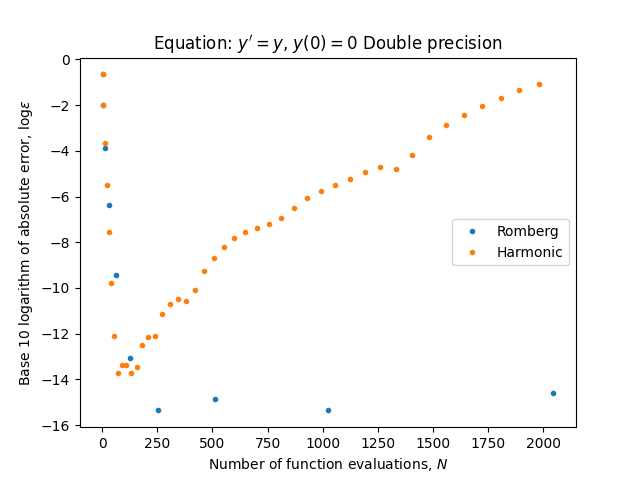
\includegraphics[scale=0.45]{../results/emr_plots/exp_growth.png}
\end{minipage}
\begin{minipage}{0.45\textwidth}
\centering
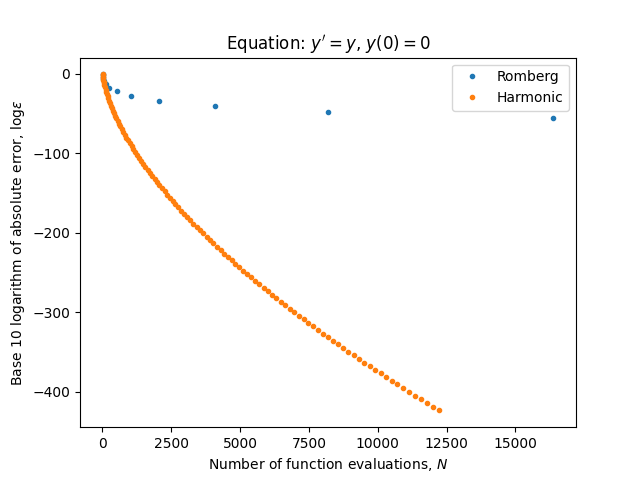
\includegraphics[scale=0.45]{../results/emr_plots/exp_growth_hp.png}
\end{minipage}
\end{figure}

\begin{figure}[H]
\centering
\begin{minipage}{0.45\textwidth}
\centering
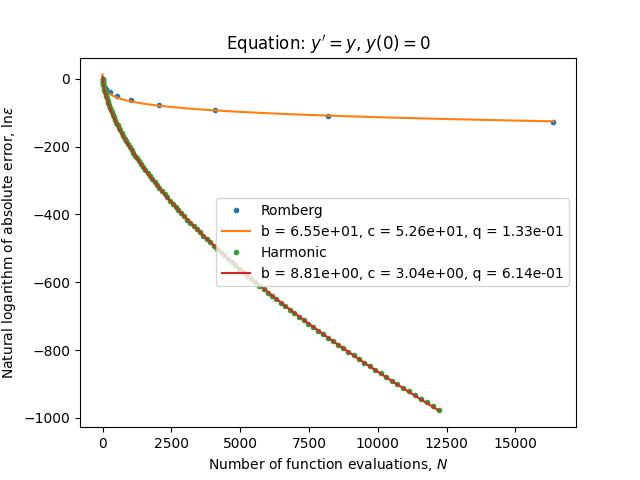
\includegraphics[scale=0.45]{../results/emr_plots/exp_growth_hp_trend.png}
\end{minipage}
\begin{minipage}{0.45\textwidth}
\centering
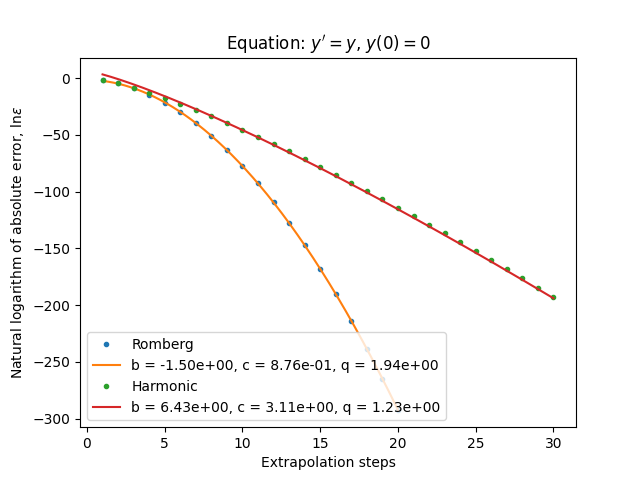
\includegraphics[scale=0.45]{../results/emr_plots/exp_growth_hp_steps.png}
\end{minipage}
\end{figure}

\begin{figure}[H]
\centering
\begin{minipage}{0.45\textwidth}
\centering
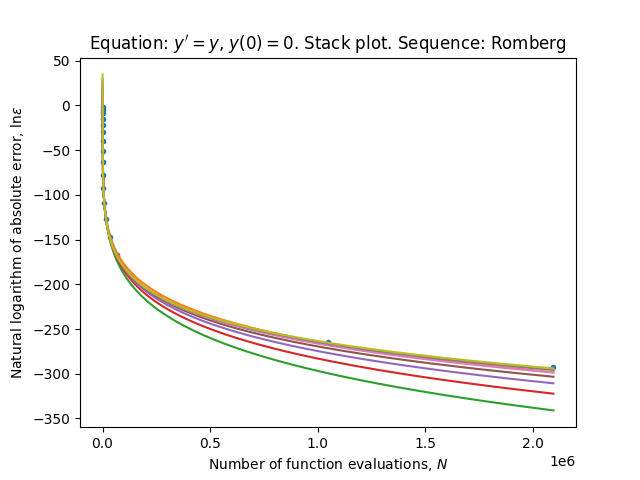
\includegraphics[scale=0.45]{../results/emr_plots/exp_growth_hp_romberg_stack.png}
\end{minipage}
\begin{minipage}{0.45\textwidth}
\centering
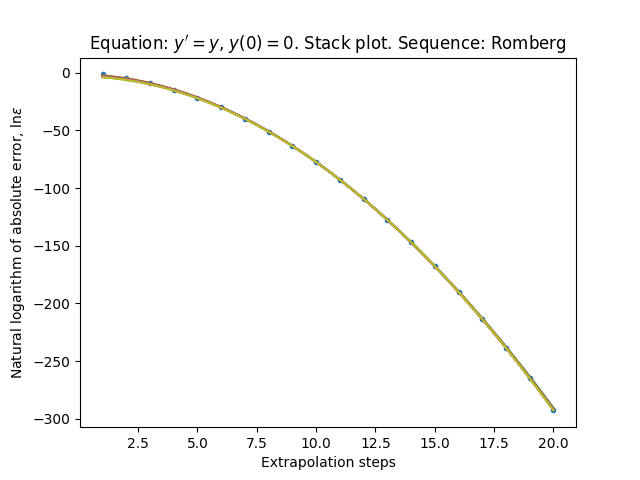
\includegraphics[scale=0.45]{../results/emr_plots/exp_growth_hp_romberg_steps_stack.png}
\end{minipage}
\end{figure}

\begin{figure}[H]
\centering
\begin{minipage}{0.45\textwidth}
\centering
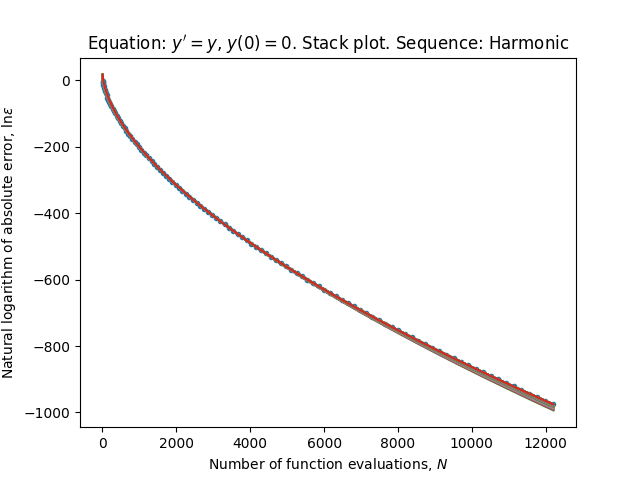
\includegraphics[scale=0.45]{../results/emr_plots/exp_growth_hp_harmonic_stack.png}
\end{minipage}
\begin{minipage}{0.45\textwidth}
\centering
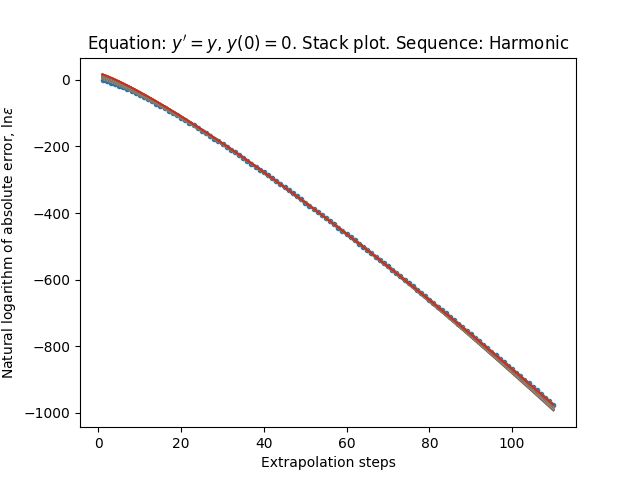
\includegraphics[scale=0.45]{../results/emr_plots/exp_growth_hp_harmonic_steps_stack.png}
\end{minipage}
\end{figure}

\begin{table}[H]
    \centering
    \small
    \begin{tabular}{c||c|c|c|c|c|c|c|c}
Sequence & \(A\)-mean & \(A\)-var & \(c\)-mean & \(c\)-var & \(q\)-mean & \(q\)-var & \(\rho_{\operatorname{lin}}\) & \(\rho_{\ln}\)\\\hline
\rowcolor{red}
Romberg & \(6.231\cdot 10^{65}\) & \(6\) & \(71.92\) & \(0.1174\) & \(0.1236\) & \(0.03122\) & \(1.415\cdot 10^8\) & \(0.0006922\) \\
\rowcolor{yellow}
Harmonic & \(1.204\cdot 10^9\) & \(6.365\) & \(3.264\) & \(0.005221\) & \(0.6081\) & \(0.0001653\) & \(8.428\cdot 10^4\) & \(5.564\cdot 10^{-6}\) \\
\rowcolor{green}
Romberg & \(0.0873\) & \(0.2223\) & \(0.841\) & \(0.0009203\) & \(1.95\) & \(2.797\cdot 10^{-5}\) & \(0.3309\) & \(4.499\cdot 10^{-6}\) \\
\rowcolor{yellow}
Harmonic & \(3.805\cdot 10^7\) & \(6.024\) & \(3.309\) & \(0.004502\) & \(1.214\) & \(0.0001425\) & \(1.574\cdot 10^4\) & \(4.503\cdot 10^{-6}\) \\
    \end{tabular}
    \label{tab:my_label}
\end{table}

The Harmonic sequence performes better. We get down to machine level precision using either sequence in double precision arithmetic.\\

We clearly have exponential convergence in the number of steps for the Romberg sequence and the fitting for the Harmonic sequence seems nice but we though have very big values for \(A\).

\subsection{Logistic curve}

Then we will consider the following initial value problem
\begin{equation}\label{43}
y'(x) = y(x)(1-y(x)),\quad y(0) = 1/2, \quad x\in [0,1]
\end{equation}

whose solution is the sigmoid function
\[
\sigma(x) = \frac{1}{1 + e^{-x}}
\]
which is analytic.

\begin{figure}[H]
\centering
\begin{minipage}{0.45\textwidth}
\centering
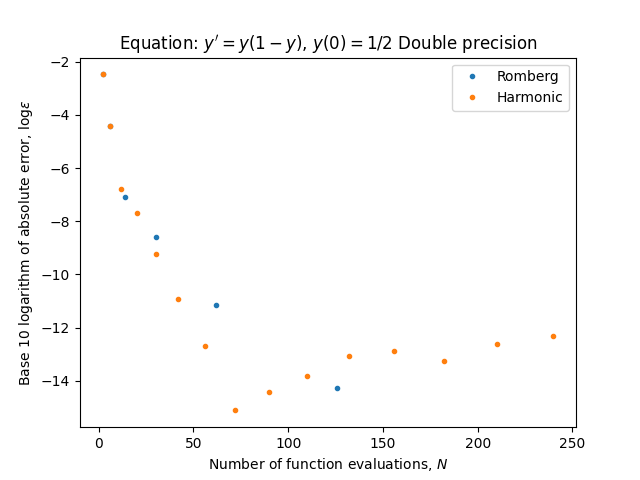
\includegraphics[scale=0.45]{../results/emr_plots/logistic.png}
\end{minipage}
\begin{minipage}{0.45\textwidth}
\centering
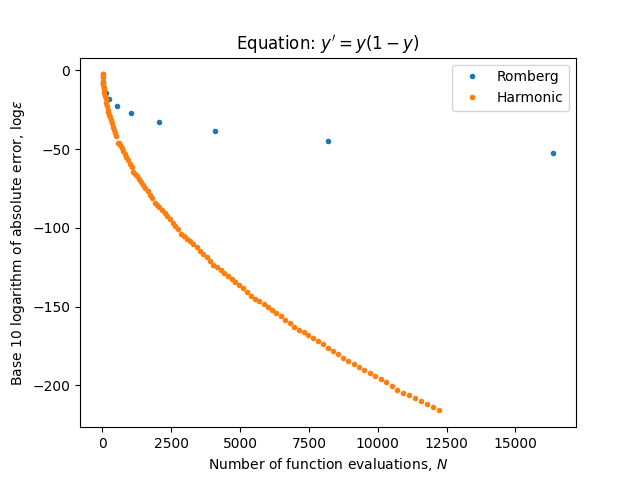
\includegraphics[scale=0.45]{../results/emr_plots/logistic_hp.png}
\end{minipage}
\end{figure}

\begin{figure}[H]
\centering
\begin{minipage}{0.45\textwidth}
\centering
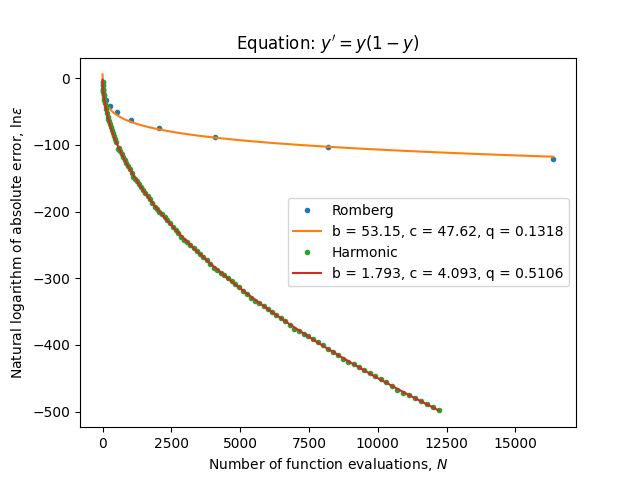
\includegraphics[scale=0.45]{../results/emr_plots/logistic_hp_trend.png}
\end{minipage}
\begin{minipage}{0.45\textwidth}
\centering
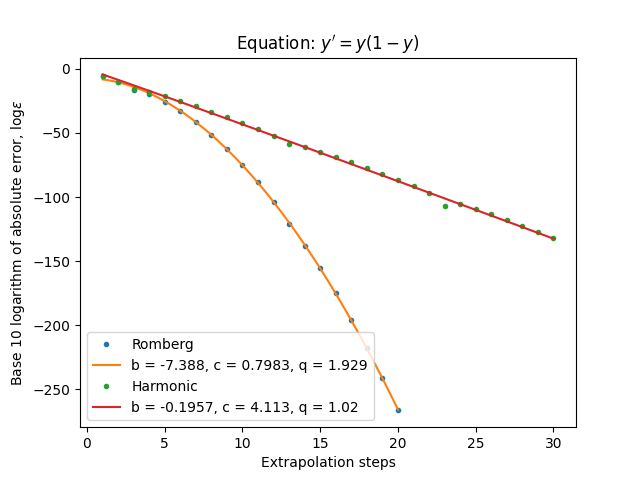
\includegraphics[scale=0.45]{../results/emr_plots/logistic_hp_steps.png}
\end{minipage}
\end{figure}

\begin{figure}[H]
\centering
\begin{minipage}{0.45\textwidth}
\centering
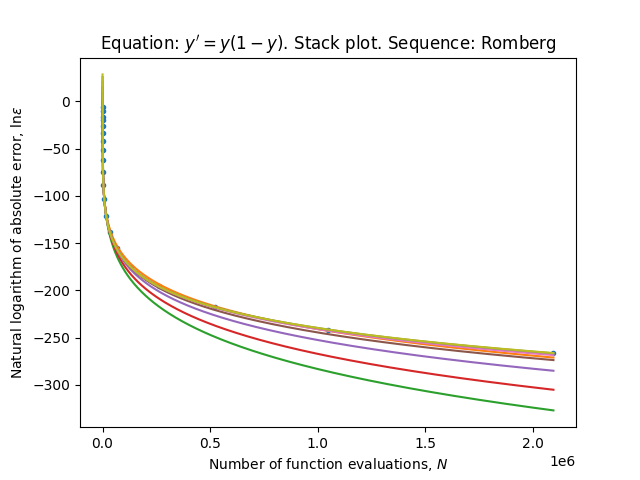
\includegraphics[scale=0.45]{../results/emr_plots/logistic_hp_romberg_stack.png}
\end{minipage}
\begin{minipage}{0.45\textwidth}
\centering
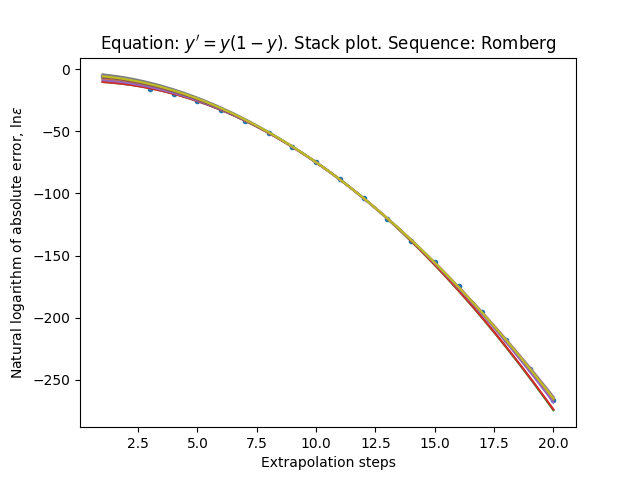
\includegraphics[scale=0.45]{../results/emr_plots/logistic_hp_romberg_steps_stack.png}
\end{minipage}
\end{figure}

\begin{figure}[H]
\centering
\begin{minipage}{0.45\textwidth}
\centering
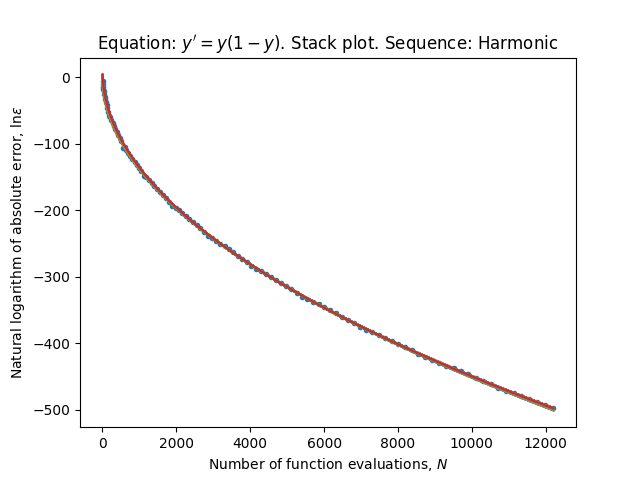
\includegraphics[scale=0.45]{../results/emr_plots/logistic_hp_harmonic_stack.png}
\end{minipage}
\begin{minipage}{0.45\textwidth}
\centering
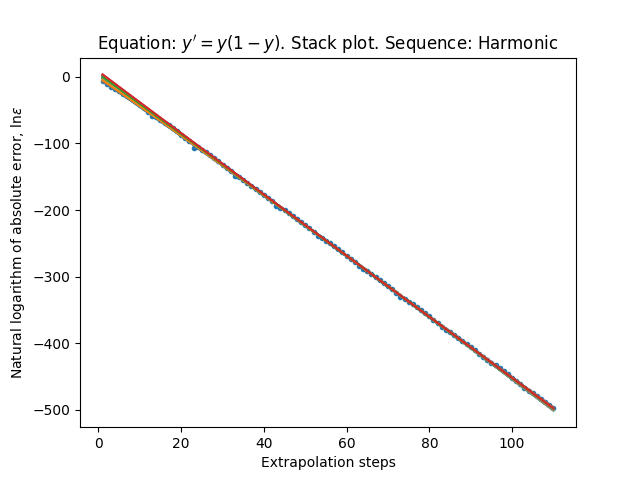
\includegraphics[scale=0.45]{../results/emr_plots/logistic_hp_harmonic_steps_stack.png}
\end{minipage}
\end{figure}

\begin{table}[H]
    \centering
    \small
    \begin{tabular}{c||c|c|c|c|c|c|c|c}
Sequence & \(A\)-mean & \(A\)-var & \(c\)-mean & \(c\)-var & \(q\)-mean & \(q\)-var & \(\rho_{\operatorname{lin}}\) & \(\rho_{\ln}\)\\\hline
\rowcolor{red}
Romberg & \(8.848\cdot 10^{63}\) & \(6\) & \(70.69\) & \(0.1952\) & \(0.1226\) & \(0.0637\) & \(6.36\cdot 10^5\) & \(0.0006121\) \\
\rowcolor{green}
Harmonic & \(2510\) & \(9.384\) & \(4.249\) & \(0.00357\) & \(0.5073\) & \(0.0001329\) & \(18.59\) & \(1.332\cdot 10^{-5}\) \\
\rowcolor{green}
Romberg & \(0.01026\) & \(1.856\) & \(0.814\) & \(0.03122\) & \(1.932\) & \(0.001091\) & \(0.839\) & \(4.568\cdot 10^{-5}\) \\
\rowcolor{green}
Harmonic & \(257.8\) & \(9.223\) & \(4.256\) & \(0.003464\) & \(1.014\) & \(0.0001294\) & \(9.348\) & \(1.304\cdot 10^{-5}\) \\
    \end{tabular}
    \label{tab:my_label}
\end{table}

The harmonic sequence performes better and we get down to machine level precisision using either sequence, in double precision.\\

We seem to have exponential convergence in the number of steps for the Romberg sequence and the models fit well for the harmonic sequence.\\

\subsection{Tangens}

Now we will consider the following equation
\begin{equation}
y'(x) = 1 + y(x)^2, \quad y(0) = 0,\quad x\in [0,1]
\end{equation}

whose solution is 
\[
y(x) \coloneqq \tan(x)
\]
which is meromorphic and we are quite far from singularites.

\begin{figure}[H]
\centering
\begin{minipage}{0.45\textwidth}
\centering
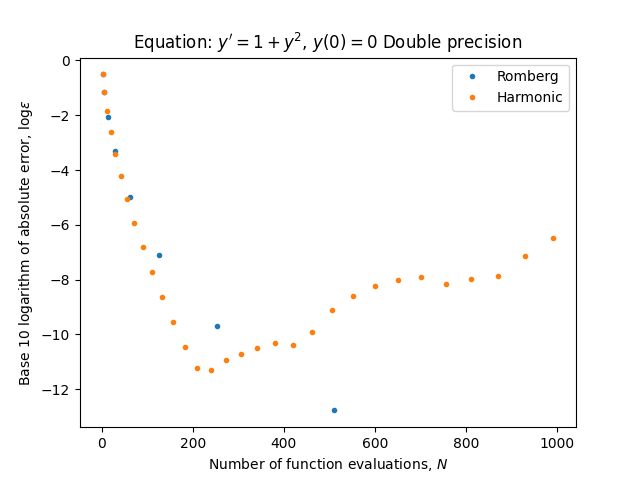
\includegraphics[scale=0.45]{../results/emr_plots/tangens.png}
\end{minipage}
\begin{minipage}{0.45\textwidth}
\centering
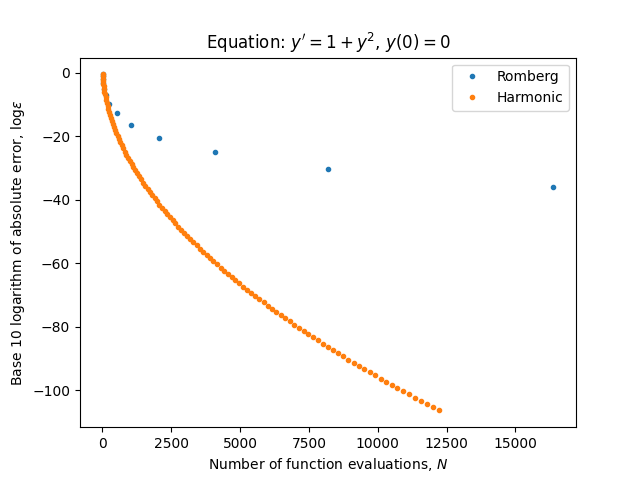
\includegraphics[scale=0.45]{../results/emr_plots/tangens_hp.png}
\end{minipage}
\end{figure}

\begin{figure}[H]
\centering
\begin{minipage}{0.45\textwidth}
\centering
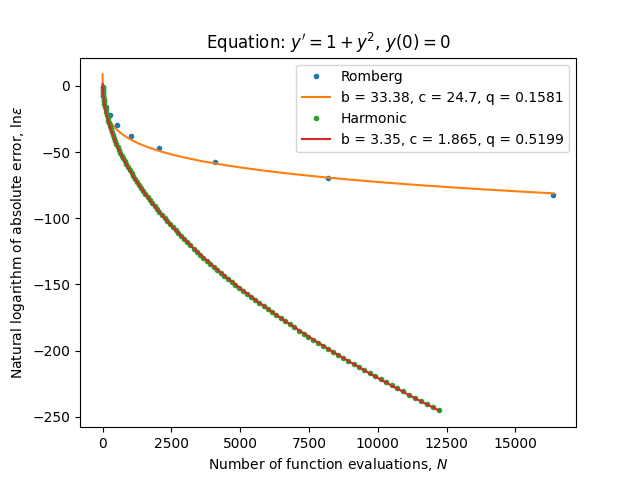
\includegraphics[scale=0.45]{../results/emr_plots/tangens_hp_trend.png}
\end{minipage}
\begin{minipage}{0.45\textwidth}
\centering
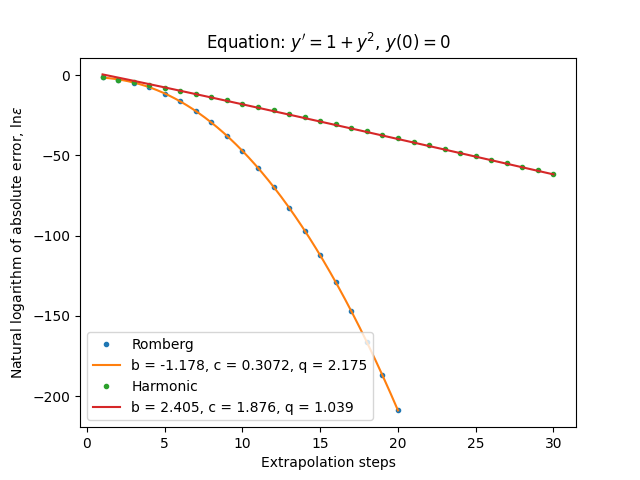
\includegraphics[scale=0.45]{../results/emr_plots/tangens_hp_steps.png}
\end{minipage}
\end{figure}

\begin{figure}[H]
\centering
\begin{minipage}{0.45\textwidth}
\centering
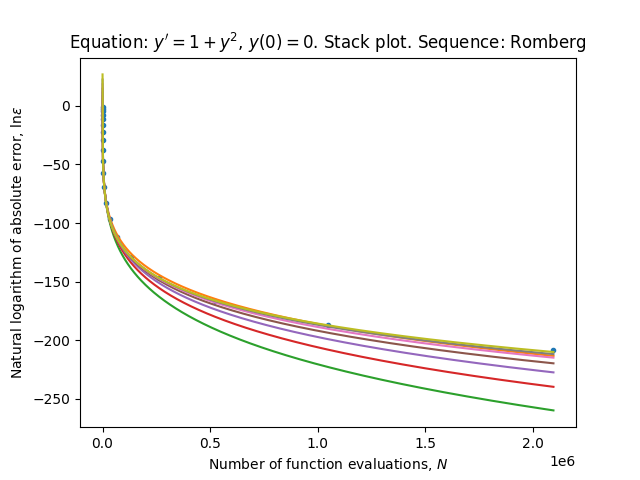
\includegraphics[scale=0.45]{../results/emr_plots/tangens_hp_romberg_stack.png}
\end{minipage}
\begin{minipage}{0.45\textwidth}
\centering
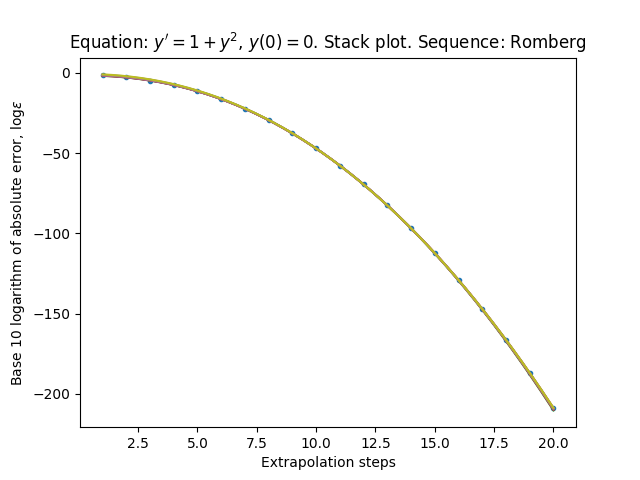
\includegraphics[scale=0.45]{../results/emr_plots/tangens_hp_romberg_steps_stack.png}
\end{minipage}
\end{figure}

\begin{figure}[H]
\centering
\begin{minipage}{0.45\textwidth}
\centering
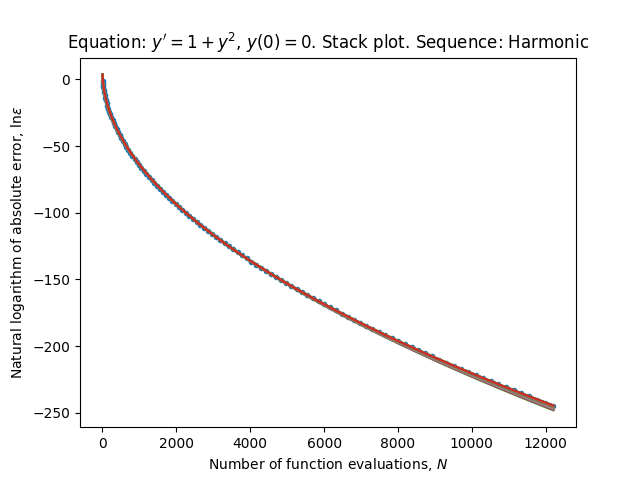
\includegraphics[scale=0.45]{../results/emr_plots/tangens_hp_harmonic_stack.png}
\end{minipage}
\begin{minipage}{0.45\textwidth}
\centering
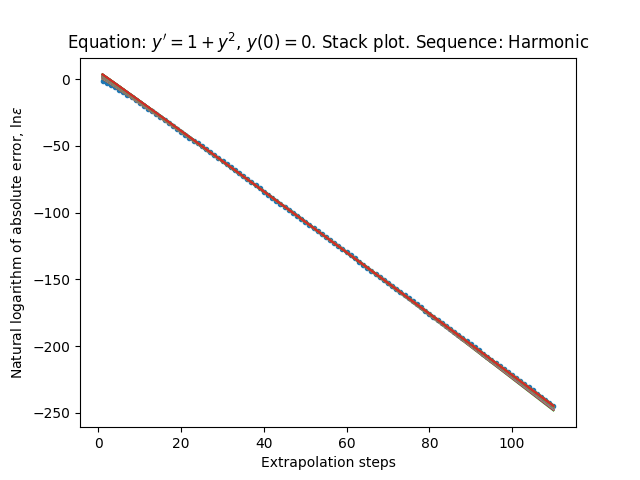
\includegraphics[scale=0.45]{../results/emr_plots/tangens_hp_harmonic_steps_stack.png}
\end{minipage}
\end{figure}

\begin{table}[H]
    \centering
    \small
    \begin{tabular}{c||c|c|c|c|c|c|c|c}
Sequence & \(A\)-mean & \(A\)-var & \(c\)-mean & \(c\)-var & \(q\)-mean & \(q\)-var & \(\rho_{\operatorname{lin}}\) & \(\rho_{\ln}\)\\\hline
\rowcolor{red}
Romberg & \(9.496\cdot 10^{36}\) & \(6\) & \(33.25\) & \(0.1689\) & \(0.1523\) & \(0.03648\) & \(1.13\cdot 10^6\) & \(0.0009519\) \\
\rowcolor{green}
Harmonic & \(358.8\) & \(0.5652\) & \(2.017\) & \(0.002488\) & \(0.5127\) & \(0.000109\) & \(27.95\) & \(5.92\cdot 10^{-6}\) \\
\rowcolor{green}
Romberg & \(0.3476\) & \(0.1097\) & \(0.3039\) & \(0.001043\) & \(2.18\) & \(2.579\cdot 10^{-5}\) & \(0.06654\) & \(1.294\cdot 10^{-6}\) \\
\rowcolor{green}
Harmonic & \(121.5\) & \(0.5373\) & \(2.021\) & \(0.002309\) & \(1.025\) & \(0.0001013\) & \(19.67\) & \(5.328\cdot 10^{-6}\) \\
    \end{tabular}
    \label{tab:my_label}
\end{table}

The harmonic sequence performes better and we get down to machine level precision in double precision arithmetic, using either sequence.\\

Here we clearly have exponential convergence in the number of steps for the Romberg sequence and the fit is also very nice for the harmonic sequence.

\subsection{The logarithm}

Now we will consider the following initial value problem:

\begin{equation}
y'(t) = \exp(-y(t)), \quad y(0) = \ln(a), \quad t\in [0,1].
\end{equation}

whose solution is 

\[
y(t) = \ln(a + t).
\]

The solution is analytic on but with a singularity on the closed horizontal ray from \(-a\) to \(-\infty\).

\subsubsection{\(a = 1\)}

\begin{figure}[H]
\centering
\begin{minipage}{0.45\textwidth}
\centering
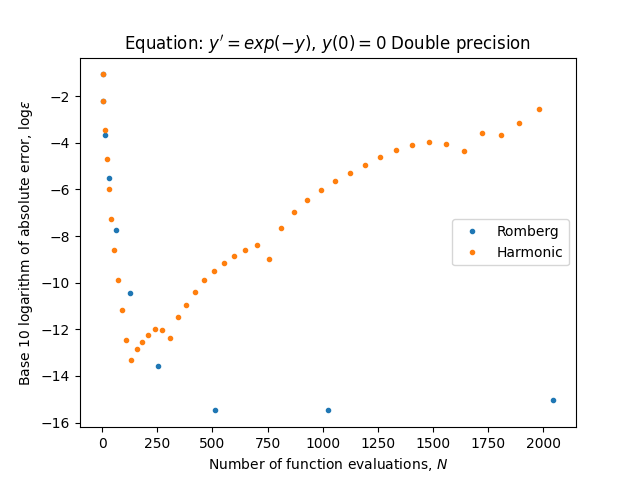
\includegraphics[scale=0.45]{../results/emr_plots/ln_e0.png}
\end{minipage}
\begin{minipage}{0.45\textwidth}
\centering
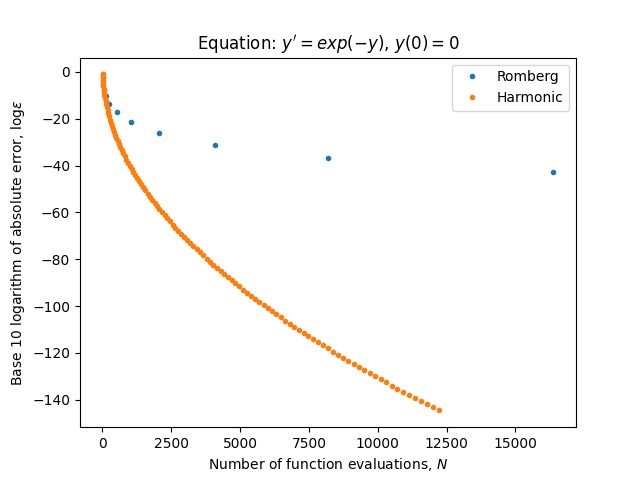
\includegraphics[scale=0.45]{../results/emr_plots/ln_e0_hp.png}
\end{minipage}
\end{figure}

\begin{figure}[H]
\centering
\begin{minipage}{0.45\textwidth}
\centering
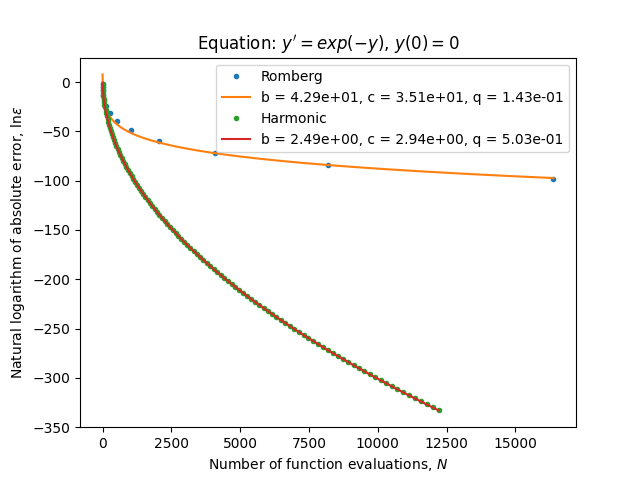
\includegraphics[scale=0.45]{../results/emr_plots/ln_e0_hp_trend.png}
\end{minipage}
\begin{minipage}{0.45\textwidth}
\centering
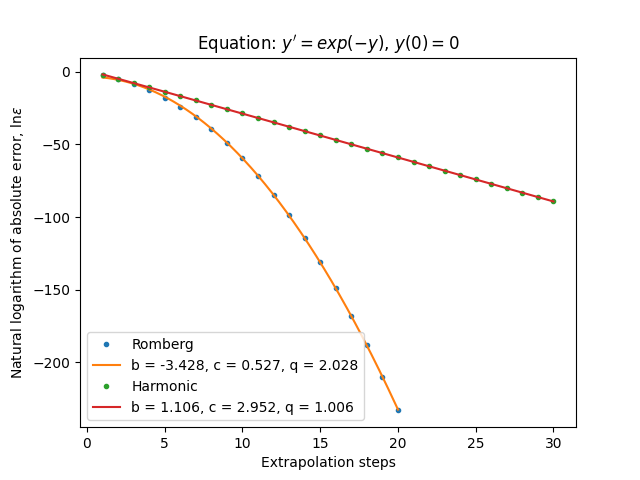
\includegraphics[scale=0.45]{../results/emr_plots/ln_e0_hp_steps.png}
\end{minipage}
\end{figure}

\begin{figure}[H]
\centering
\begin{minipage}{0.45\textwidth}
\centering
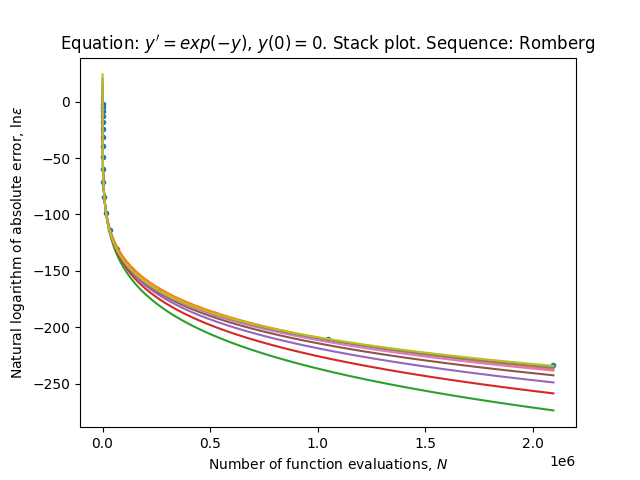
\includegraphics[scale=0.45]{../results/emr_plots/ln_e0_hp_romberg_stack.png}
\end{minipage}
\begin{minipage}{0.45\textwidth}
\centering
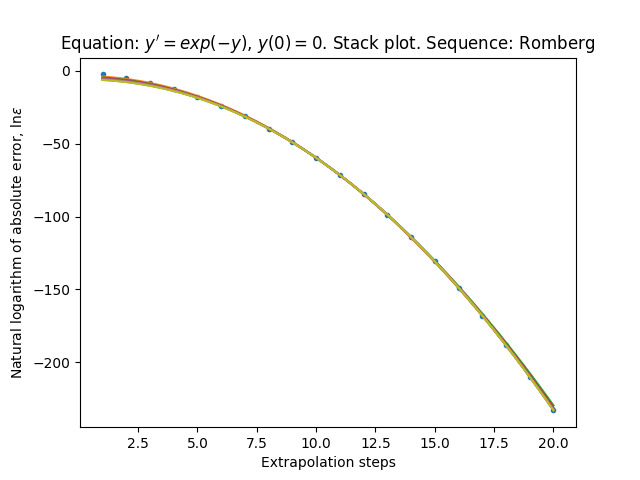
\includegraphics[scale=0.45]{../results/emr_plots/ln_e0_hp_romberg_steps_stack.png}
\end{minipage}
\end{figure}

\begin{figure}[H]
\centering
\begin{minipage}{0.45\textwidth}
\centering
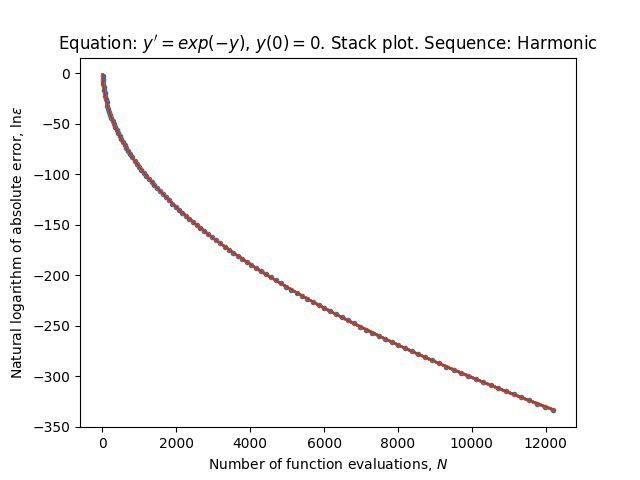
\includegraphics[scale=0.45]{../results/emr_plots/ln_e0_hp_harmonic_stack.png}
\end{minipage}
\begin{minipage}{0.45\textwidth}
\centering
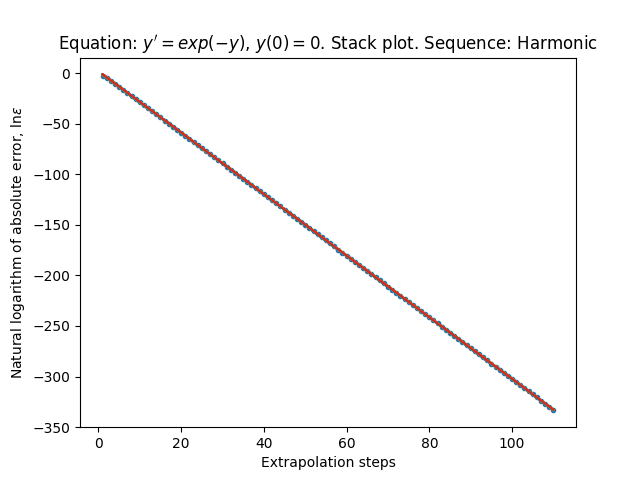
\includegraphics[scale=0.45]{../results/emr_plots/ln_e0_hp_harmonic_steps_stack.png}
\end{minipage}
\end{figure}

\begin{table}[H]
    \centering
    \small
    \begin{tabular}{c||c|c|c|c|c|c|c|c}
Sequence & \(A\)-mean & \(A\)-var & \(c\)-mean & \(c\)-var & \(q\)-mean & \(q\)-var & \(\rho_{\operatorname{lin}}\) & \(\rho_{\ln}\)\\\hline
\rowcolor{red}
Romberg & \(4.885\cdot 10^{42}\) & \(6\) & \(45.32\) & \(0.1197\) & \(0.1365\) & \(0.02779\) & \(5.241\cdot 10^5\) & \(0.0006028\) \\
\rowcolor{green}
Harmonic & \(21.43\) & \(0.04237\) & \(2.986\) & \(6.169\cdot 10^{-5}\) & \(0.5019\) & \(2.669\cdot 10^{-6}\) & \(1.32\) & \(2.916\cdot 10^{-7}\) \\
\rowcolor{green}
Romberg & \(0.007492\) & \(0.413\) & \(0.4813\) & \(0.003324\) & \(2.056\) & \(9.134\cdot 10^{-5}\) & \(0.6043\) & \(2.141\cdot 10^{-5}\) \\
\rowcolor{green}
Harmonic & \(4.89\) & \(0.03478\) & \(2.989\) & \(4.918\cdot 10^{-5}\) & \(1.004\) & \(2.126\cdot 10^{-6}\) & \(0.6747\) & \(1.905\cdot 10^{-7}\) \\
    \end{tabular}
    \label{tab:my_label}
\end{table}

Here the harmonic sequence works better.\\

We have exponential convergence in the number of evaluations and the number of steps for the harmonic sequence and we have exponential convergence in the number of steps for the Romberg sequence.

\subsubsection{\(a = e^{-1}\)}
\begin{figure}[H]
\centering
\begin{minipage}{0.45\textwidth}
\centering
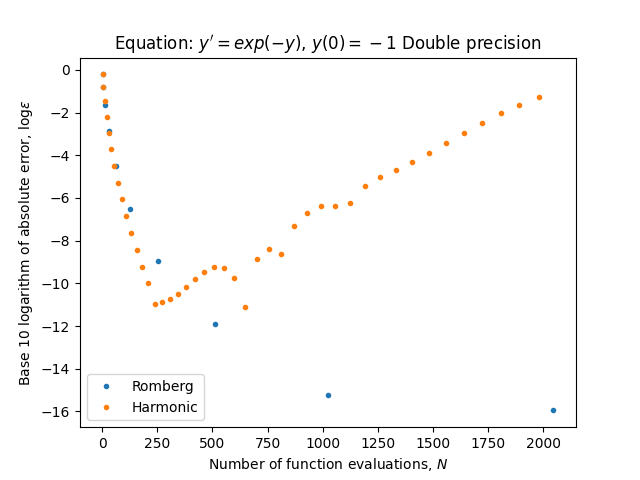
\includegraphics[scale=0.45]{../results/emr_plots/ln_em1.png}
\end{minipage}
\begin{minipage}{0.45\textwidth}
\centering
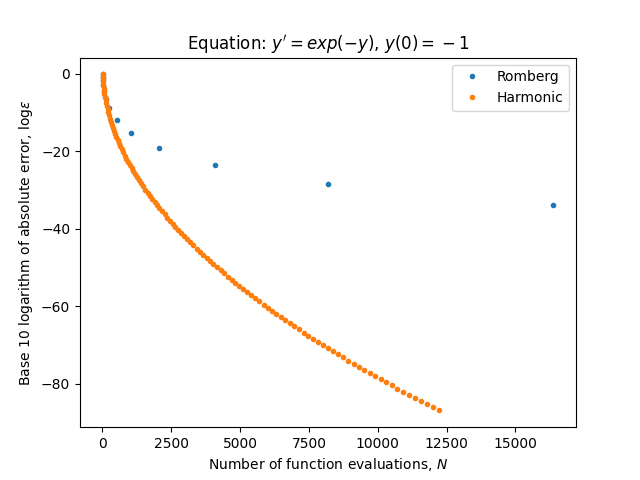
\includegraphics[scale=0.45]{../results/emr_plots/ln_em1_hp.png}
\end{minipage}
\end{figure}

\begin{figure}[H]
\centering
\begin{minipage}{0.45\textwidth}
\centering
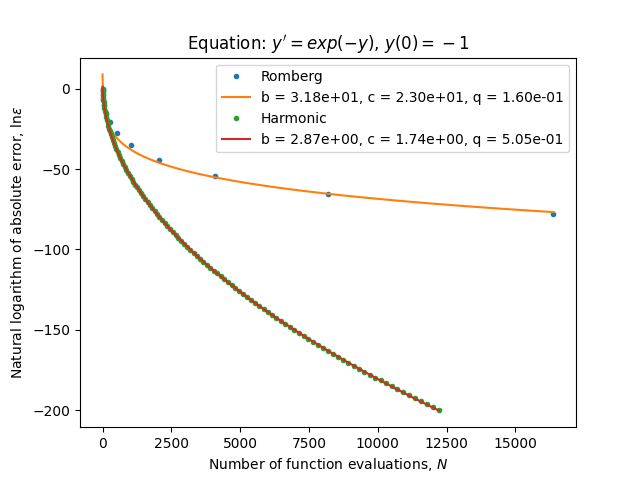
\includegraphics[scale=0.45]{../results/emr_plots/ln_em1_hp_trend.png}
\end{minipage}
\begin{minipage}{0.45\textwidth}
\centering
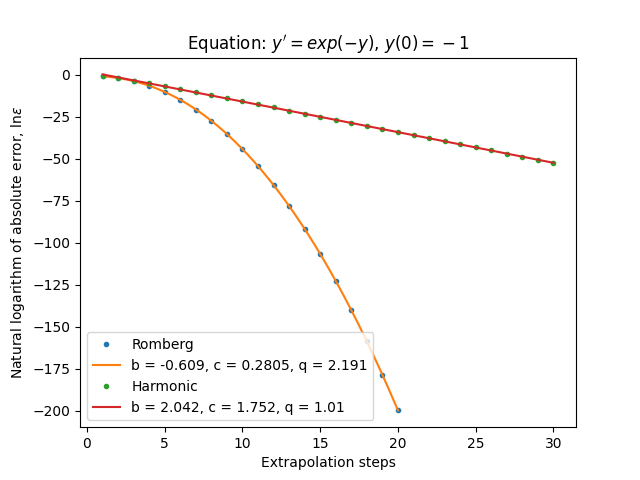
\includegraphics[scale=0.45]{../results/emr_plots/ln_em1_hp_steps.png}
\end{minipage}
\end{figure}

\begin{figure}[H]
\centering
\begin{minipage}{0.45\textwidth}
\centering
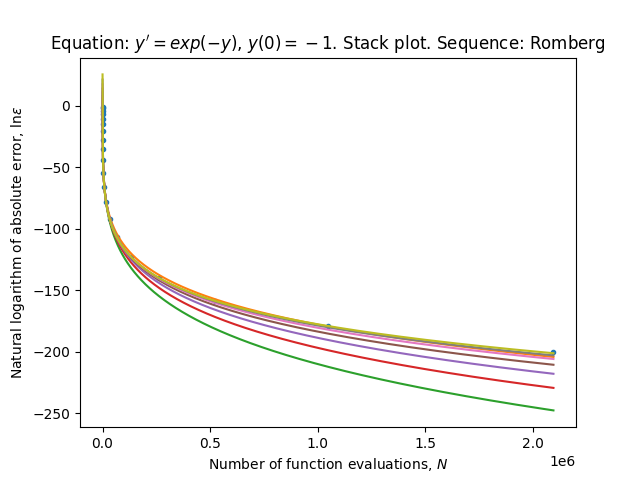
\includegraphics[scale=0.45]{../results/emr_plots/ln_em1_hp_romberg_stack.png}
\end{minipage}
\begin{minipage}{0.45\textwidth}
\centering
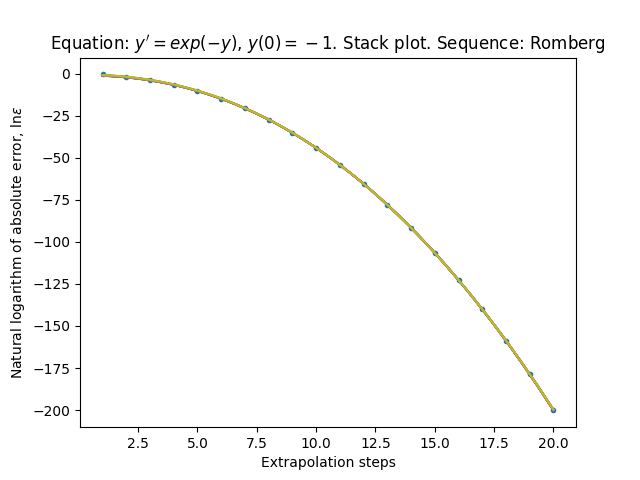
\includegraphics[scale=0.45]{../results/emr_plots/ln_em1_hp_romberg_steps_stack.png}
\end{minipage}
\end{figure}

\begin{figure}[H]
\centering
\begin{minipage}{0.45\textwidth}
\centering
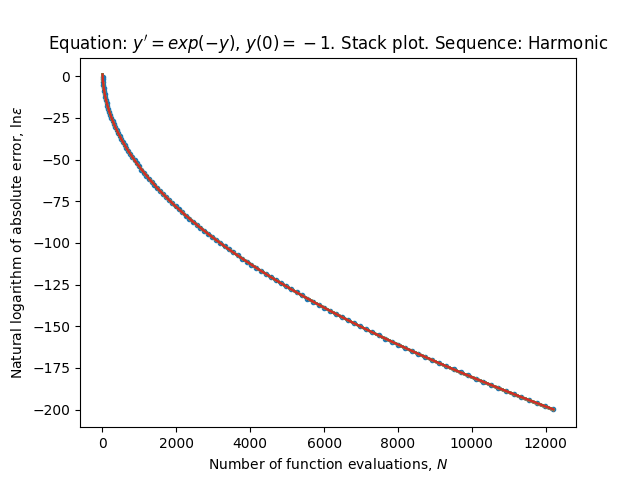
\includegraphics[scale=0.45]{../results/emr_plots/ln_em1_hp_harmonic_stack.png}
\end{minipage}
\begin{minipage}{0.45\textwidth}
\centering
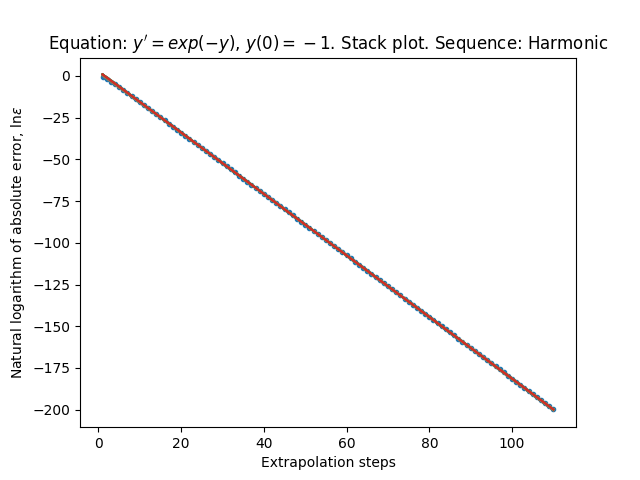
\includegraphics[scale=0.45]{../results/emr_plots/ln_em1_hp_harmonic_steps_stack.png}
\end{minipage}
\end{figure}

\begin{table}[H]
    \centering
    \small
    \begin{tabular}{c||c|c|c|c|c|c|c|c}
Sequence & \(A\)-mean & \(A\)-var & \(c\)-mean & \(c\)-var & \(q\)-mean & \(q\)-var & \(\rho_{\operatorname{lin}}\) & \(\rho_{\ln}\)\\\hline
\rowcolor{red}
Romberg & \(1.253\cdot 10^{34}\) & \(6\) & \(30.35\) & \(0.163\) & \(0.1548\) & \(0.03379\) & \(4.863\cdot 10^5\) & \(0.0009135\) \\
\rowcolor{green}
Harmonic & \(30.61\) & \(0.03646\) & \(1.788\) & \(0.0001346\) & \(0.5031\) & \(5.761\cdot 10^{-6}\) & \(1.864\) & \(9.42\cdot 10^{-7}\) \\
\rowcolor{green}
Romberg & \(0.4234\) & \(0.02508\) & \(0.2721\) & \(0.0001868\) & \(2.202\) & \(4.231\cdot 10^{-6}\) & \(0.1032\) & \(1.729\cdot 10^{-6}\) \\
\rowcolor{green}
Harmonic & \(12.56\) & \(0.03136\) & \(1.79\) & \(0.0001139\) & \(1.006\) & \(4.872\cdot 10^{-6}\) & \(1.294\) & \(7.415\cdot 10^{-7}\) \\
    \end{tabular}
    \label{tab:my_label}
\end{table}

Here the same comments apply as when \(a = 1\).

\subsubsection{\(a = e^{-2}\)}

\begin{figure}[H]
\centering
\begin{minipage}{0.45\textwidth}
\centering
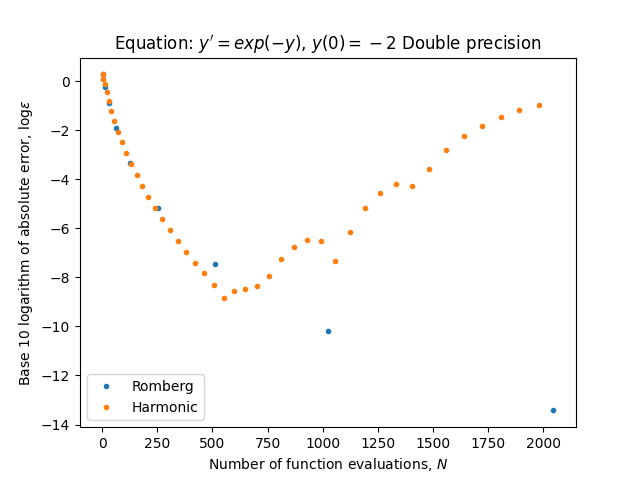
\includegraphics[scale=0.45]{../results/emr_plots/ln_em2.png}
\end{minipage}
\begin{minipage}{0.45\textwidth}
\centering
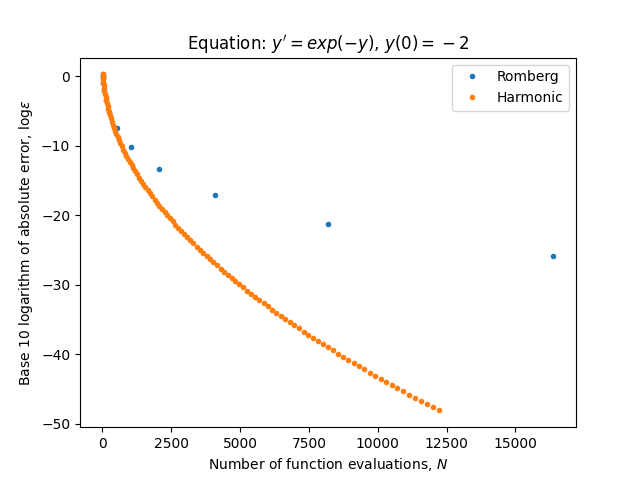
\includegraphics[scale=0.45]{../results/emr_plots/ln_em2_hp.png}
\end{minipage}
\end{figure}

\begin{figure}[H]
\centering
\begin{minipage}{0.45\textwidth}
\centering
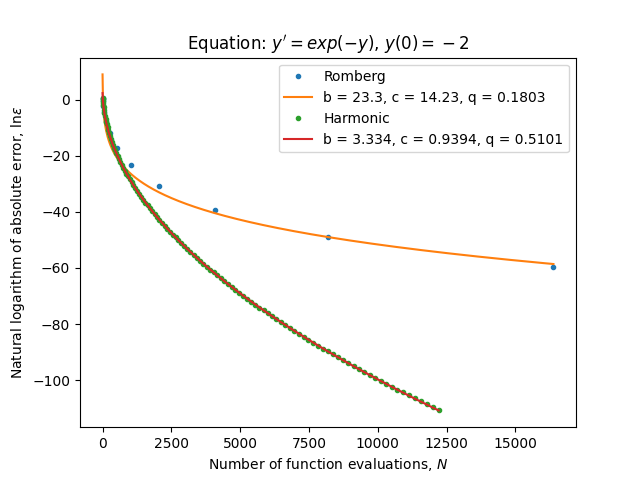
\includegraphics[scale=0.45]{../results/emr_plots/ln_em2_hp_trend.png}
\end{minipage}
\begin{minipage}{0.45\textwidth}
\centering
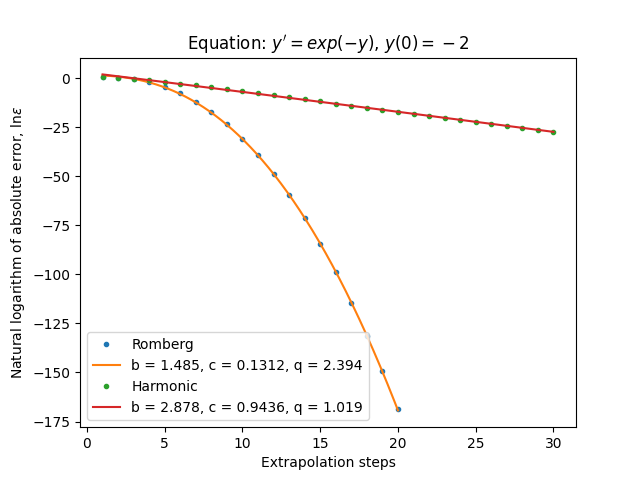
\includegraphics[scale=0.45]{../results/emr_plots/ln_em2_hp_steps.png}
\end{minipage}
\end{figure}

\begin{figure}[H]
\centering
\begin{minipage}{0.45\textwidth}
\centering
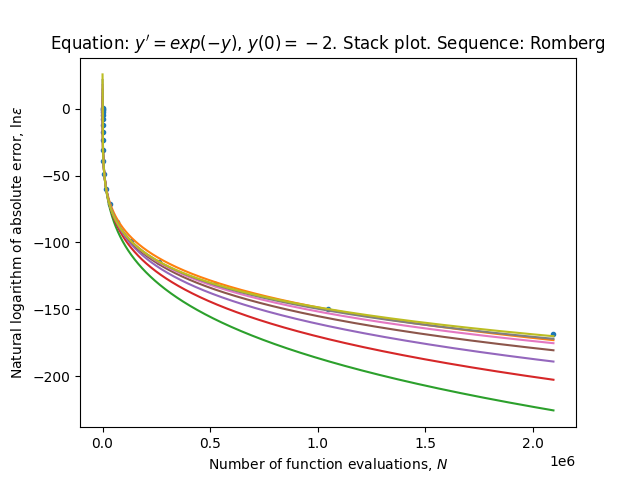
\includegraphics[scale=0.45]{../results/emr_plots/ln_em2_hp_romberg_stack.png}
\end{minipage}
\begin{minipage}{0.45\textwidth}
\centering
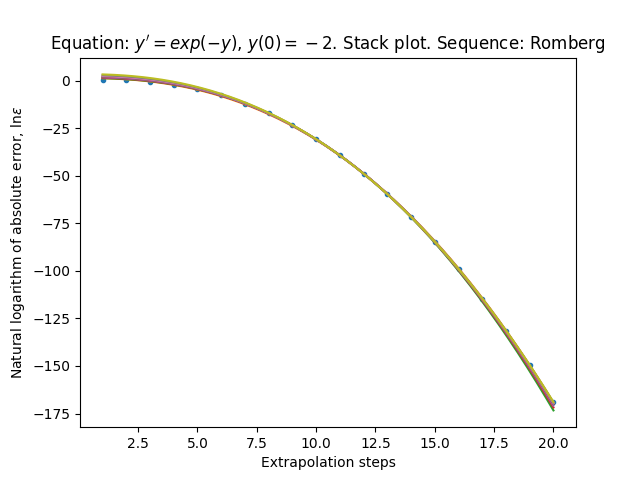
\includegraphics[scale=0.45]{../results/emr_plots/ln_em2_hp_romberg_steps_stack.png}
\end{minipage}
\end{figure}

\begin{figure}[H]
\centering
\begin{minipage}{0.45\textwidth}
\centering
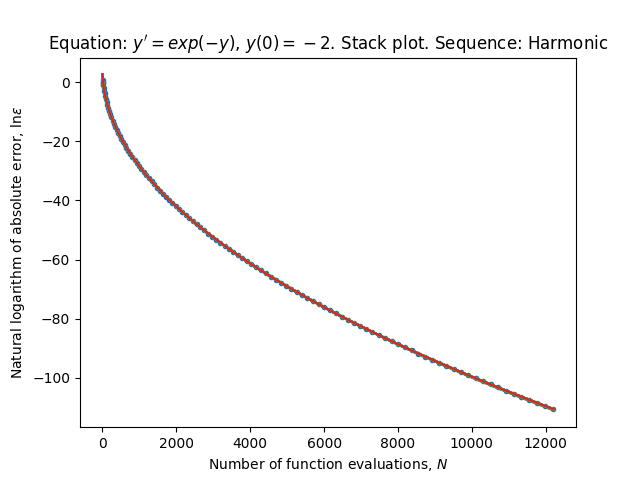
\includegraphics[scale=0.45]{../results/emr_plots/ln_em2_hp_harmonic_stack.png}
\end{minipage}
\begin{minipage}{0.45\textwidth}
\centering
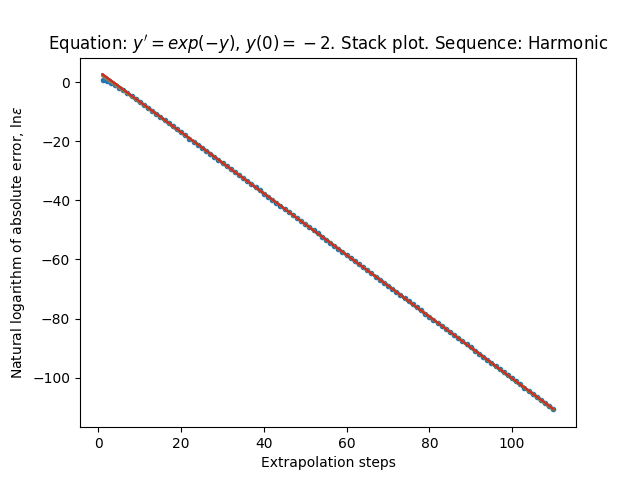
\includegraphics[scale=0.45]{../results/emr_plots/ln_em2_hp_harmonic_steps_stack.png}
\end{minipage}
\end{figure}

\begin{table}[H]
    \centering
    \small
    \begin{tabular}{c||c|c|c|c|c|c|c|c}
Sequence & \(A\)-mean & \(A\)-var & \(c\)-mean & \(c\)-var & \(q\)-mean & \(q\)-var & \(\rho_{\operatorname{lin}}\) & \(\rho_{\ln}\)\\\hline
\rowcolor{red}
Romberg & \(6.703\cdot 10^{26}\) & \(6\) & \(19.26\) & \(0.2229\) & \(0.1773\) & \(0.04097\) & \(2.919\cdot 10^5\) & \(0.001426\) \\
\rowcolor{green}
Harmonic & \(52.85\) & \(0.01529\) & \(0.9931\) & \(0.0001445\) & \(0.5047\) & \(6.004\cdot 10^{-6}\) & \(5.014\) & \(7.709\cdot 10^{-6}\) \\
\rowcolor{green}
Romberg & \(13.84\) & \(0.5067\) & \(0.138\) & \(0.01003\) & \(2.383\) & \(0.0002168\) & \(0.7745\) & \(2.073\cdot 10^{-5}\) \\
\rowcolor{green}
Harmonic & \(32.1\) & \(0.01319\) & \(0.9945\) & \(0.0001227\) & \(1.009\) & \(5.087\cdot 10^{-6}\) & \(4.245\) & \(7.068\cdot 10^{-6}\) \\
    \end{tabular}
    \label{tab:my_label}
\end{table}

Here the same comments apply as when \(a = 1\).

\subsubsection{\(a = e^{-4}\)}

\begin{figure}[H]
\centering
\begin{minipage}{0.45\textwidth}
\centering
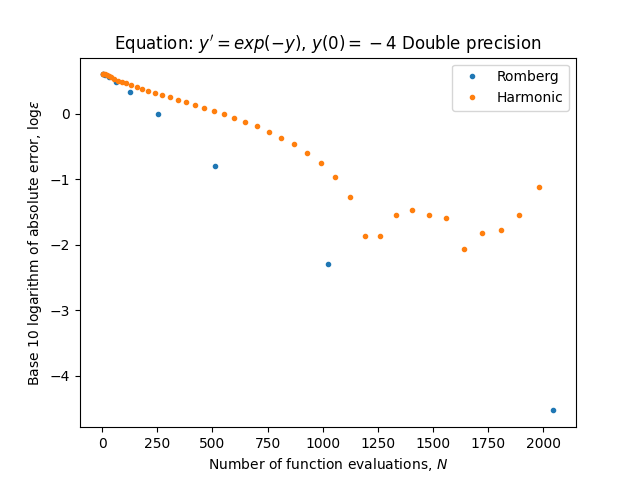
\includegraphics[scale=0.45]{../results/emr_plots/ln_em4.png}
\end{minipage}
\begin{minipage}{0.45\textwidth}
\centering
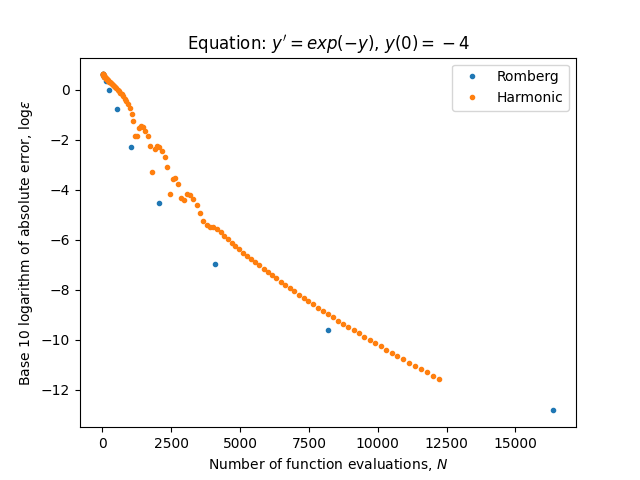
\includegraphics[scale=0.45]{../results/emr_plots/ln_em4_hp.png}
\end{minipage}
\end{figure}

\begin{figure}[H]
\centering
\begin{minipage}{0.45\textwidth}
\centering
\includegraphics[scale=0.45]{../results/emr_plots/ln_em4_hp_trend.png}
\end{minipage}
\begin{minipage}{0.45\textwidth}
\centering
\includegraphics[scale=0.45]{../results/emr_plots/ln_em4_hp_steps.png}
\end{minipage}
\end{figure}

\begin{figure}[H]
\centering
\begin{minipage}{0.45\textwidth}
\centering
\includegraphics[scale=0.45]{../results/emr_plots/ln_em4_hp_romberg_stack.png}
\end{minipage}
\begin{minipage}{0.45\textwidth}
\centering
\includegraphics[scale=0.45]{../results/emr_plots/ln_em4_hp_romberg_steps_stack.png}
\end{minipage}
\end{figure}

\begin{figure}[H]
\centering
\begin{minipage}{0.45\textwidth}
\centering
\includegraphics[scale=0.45]{../results/emr_plots/ln_em4_hp_harmonic_stack.png}
\end{minipage}
\begin{minipage}{0.45\textwidth}
\centering
\includegraphics[scale=0.45]{../results/emr_plots/ln_em4_hp_harmonic_steps_stack.png}
\end{minipage}
\end{figure}

\begin{table}[H]
    \centering
    \small
    \begin{tabular}{c||c|c|c|c|c|c|c|c}
Sequence & \(A\)-mean & \(A\)-var & \(c\)-mean & \(c\)-var & \(q\)-mean & \(q\)-var & \(\rho_{\operatorname{lin}}\) & \(\rho_{\ln}\)\\\hline
\rowcolor{red}
Romberg & \(1.768\cdot 10^{15}\) & \(5.856\) & \(6.076\) & \(0.5152\) & \(0.2574\) & \(0.1078\) & \(7022\) & \(0.003923\) \\
\rowcolor{red}
Harmonic & \(3.118\cdot 10^{13}\) & \(28.2\) & \(1.047\) & \(2.401\) & \(0.5476\) & \(0.1796\) & \(3.262\) & \(0.003283\) \\
\rowcolor{red}
Romberg & \(1740\) & \(1.019\) & \(0.02087\) & \(0.366\) & \(3.03\) & \(0.01318\) & \(10.56\) & \(0.0007478\) \\
\rowcolor{red}
Harmonic & \(1.45\cdot 10^{13}\) & \(28.09\) & \(1.027\) & \(2.361\) & \(1.093\) & \(0.1757\) & \(3.112\) & \(0.003259\) \\
    \end{tabular}
    \label{tab:my_label}
\end{table}

Here we get much slower convergence than in the previous cases and the model does not fit in any case.

\subsubsection{\(a = e^{-6}\)}

\begin{figure}[H]
\centering
\begin{minipage}{0.45\textwidth}
\centering
\includegraphics[scale=0.45]{../results/emr_plots/ln_em6.png}
\end{minipage}
\begin{minipage}{0.45\textwidth}
\centering
\includegraphics[scale=0.45]{../results/emr_plots/ln_em6_hp.png}
\end{minipage}
\end{figure}

\begin{figure}[H]
\centering
\begin{minipage}{0.45\textwidth}
\centering
\includegraphics[scale=0.45]{../results/emr_plots/ln_em6_hp_trend.png}
\end{minipage}
\begin{minipage}{0.45\textwidth}
\centering
\includegraphics[scale=0.45]{../results/emr_plots/ln_em6_hp_steps.png}
\end{minipage}
\end{figure}

\begin{figure}[H]
\centering
\begin{minipage}{0.45\textwidth}
\centering
\includegraphics[scale=0.45]{../results/emr_plots/ln_em6_hp_romberg_stack.png}
\end{minipage}
\begin{minipage}{0.45\textwidth}
\centering
\includegraphics[scale=0.45]{../results/emr_plots/ln_em6_hp_romberg_steps_stack.png}
\end{minipage}
\end{figure}

\begin{figure}[H]
\centering
\begin{minipage}{0.45\textwidth}
\centering
\includegraphics[scale=0.45]{../results/emr_plots/ln_em6_hp_harmonic_stack.png}
\end{minipage}
\begin{minipage}{0.45\textwidth}
\centering
\includegraphics[scale=0.45]{../results/emr_plots/ln_em6_hp_harmonic_steps_stack.png}
\end{minipage}
\end{figure}

\begin{table}[H]
    \centering
    \small
    \begin{tabular}{c||c|c|c|c|c|c|c|c}
Sequence & \(A\)-mean & \(A\)-var & \(c\)-mean & \(c\)-var & \(q\)-mean & \(q\)-var & \(\rho_{\operatorname{lin}}\) & \(\rho_{\ln}\)\\\hline
\rowcolor{red}
Romberg & \(1.103\cdot 10^4\) & \(5.839\) & \(0.1695\) & \(2.457\) & \(0.6307\) & \(0.1706\) & \(6.594\) & \(0.006067\) \\
\rowcolor{red}
Harmonic & \(6.659\) & \(0.0009203\) & \(0.004057\) & \(0.1522\) & \(0.6042\) & \(0.00972\) & \(0.0003433\) & \(0.0001041\) \\
\rowcolor{red}
Romberg & \(54.13\) & \(3.259\) & \(2.868\cdot 10^{-5}\) & \(3.836\) & \(6.419\) & \(0.06706\) & \(0.662\) & \(0.002097\) \\
\rowcolor{red}
Harmonic & \(6.636\) & \(0.0008806\) & \(0.004099\) & \(0.1488\) & \(1.206\) & \(0.00939\) & \(0.0003374\) & \(0.0001024\) \\
    \end{tabular}
    \label{tab:my_label}
\end{table}

Here we do simply not get convergence towards the solution and all the models fail.

\subsection{Equation with singularity}

Now we will consider the following initial value problem:
\begin{equation}\label{46}
y'(t) = y^2(t),\quad y(0) = 1/(1+a), \quad t\in [0,1]
\end{equation}

whose solution is 
\[
y(t) = \frac{1}{1-(t-a)}.
\]
The solution is meromorphic with a pole at \(1+a\).

\subsubsection{\(a = 1\)}

\begin{figure}[H]
\centering
\begin{minipage}{0.45\textwidth}
\centering
\includegraphics[scale=0.45]{../results/emr_plots/singularity_0.png}
\end{minipage}
\begin{minipage}{0.45\textwidth}
\centering
\includegraphics[scale=0.45]{../results/emr_plots/singularity_0_hp.png}
\end{minipage}
\end{figure}

\begin{figure}[H]
\centering
\begin{minipage}{0.45\textwidth}
\centering
\includegraphics[scale=0.45]{../results/emr_plots/singularity_0_hp_trend.png}
\end{minipage}
\begin{minipage}{0.45\textwidth}
\centering
\includegraphics[scale=0.45]{../results/emr_plots/singularity_0_hp_steps.png}
\end{minipage}
\end{figure}

\begin{figure}[H]
\centering
\begin{minipage}{0.45\textwidth}
\centering
\includegraphics[scale=0.45]{../results/emr_plots/singularity_0_hp_romberg_stack.png}
\end{minipage}
\begin{minipage}{0.45\textwidth}
\centering
\includegraphics[scale=0.45]{../results/emr_plots/singularity_0_hp_romberg_steps_stack.png}
\end{minipage}
\end{figure}

\begin{figure}[H]
\centering
\begin{minipage}{0.45\textwidth}
\centering
\includegraphics[scale=0.45]{../results/emr_plots/singularity_0_hp_harmonic_stack.png}
\end{minipage}
\begin{minipage}{0.45\textwidth}
\centering
\includegraphics[scale=0.45]{../results/emr_plots/singularity_0_hp_harmonic_steps_stack.png}
\end{minipage}
\end{figure}

\begin{table}[H]
    \centering
    \small
    \begin{tabular}{c||c|c|c|c|c|c|c|c}
Sequence & \(A\)-mean & \(A\)-var & \(c\)-mean & \(c\)-var & \(q\)-mean & \(q\)-var & \(\rho_{\operatorname{lin}}\) & \(\rho_{\ln}\)\\\hline
\rowcolor{red}
Romberg & \(1.418\cdot 10^{42}\) & \(6\) & \(42.1\) & \(0.1387\) & \(0.141\) & \(0.03195\) & \(1.734\cdot 10^6\) & \(0.0007659\) \\
\rowcolor{green}
Harmonic & \(440\) & \(0.5196\) & \(2.747\) & \(0.001256\) & \(0.5092\) & \(5.472\cdot 10^{-5}\) & \(52.08\) & \(3.588\cdot 10^{-6}\) \\
\rowcolor{green}
Romberg & \(0.04186\) & \(0.03016\) & \(0.4274\) & \(0.0002961\) & \(2.091\) & \(8.21\cdot 10^{-6}\) & \(0.2758\) & \(4.731\cdot 10^{-6}\) \\
\rowcolor{green}
Harmonic & \(104.3\) & \(0.4903\) & \(2.752\) & \(0.001151\) & \(1.018\) & \(5.022\cdot 10^{-5}\) & \(34.01\) & \(3.153\cdot 10^{-6}\) \\
    \end{tabular}
    \label{tab:my_label}
\end{table}

The harmonic sequence performes better and we get almost down to machine level precision using standar double precision floating point arithmetic, with either sequence.\\

We have very nice fit for the exponential convergence in the number of steps for the Romberg sequence and also for the harmonic sequence.

\subsubsection{\(a = 10^{-2}\)}

\begin{figure}[H]
\centering
\begin{minipage}{0.45\textwidth}
\centering
\includegraphics[scale=0.45]{../results/emr_plots/singularity_2.png}
\end{minipage}
\begin{minipage}{0.45\textwidth}
\centering
\includegraphics[scale=0.45]{../results/emr_plots/singularity_2_hp.png}
\end{minipage}
\end{figure}

\begin{figure}[H]
\centering
\begin{minipage}{0.45\textwidth}
\centering
\includegraphics[scale=0.45]{../results/emr_plots/singularity_2_hp_trend.png}
\end{minipage}
\begin{minipage}{0.45\textwidth}
\centering
\includegraphics[scale=0.45]{../results/emr_plots/singularity_2_hp_steps.png}
\end{minipage}
\end{figure}

\begin{figure}[H]
\centering
\begin{minipage}{0.45\textwidth}
\centering
\includegraphics[scale=0.45]{../results/emr_plots/singularity_2_hp_romberg_stack.png}
\end{minipage}
\begin{minipage}{0.45\textwidth}
\centering
\includegraphics[scale=0.45]{../results/emr_plots/singularity_2_hp_romberg_steps_stack.png}
\end{minipage}
\end{figure}

\begin{figure}[H]
\centering
\begin{minipage}{0.45\textwidth}
\centering
\includegraphics[scale=0.45]{../results/emr_plots/singularity_2_hp_harmonic_stack.png}
\end{minipage}
\begin{minipage}{0.45\textwidth}
\centering
\includegraphics[scale=0.45]{../results/emr_plots/singularity_2_hp_harmonic_steps_stack.png}
\end{minipage}
\end{figure}

\begin{table}[H]
    \centering
    \small
    \begin{tabular}{c||c|c|c|c|c|c|c|c}
Sequence & \(A\)-mean & \(A\)-var & \(c\)-mean & \(c\)-var & \(q\)-mean & \(q\)-var & \(\rho_{\operatorname{lin}}\) & \(\rho_{\ln}\)\\\hline
\rowcolor{red}
Romberg & \(1.249\cdot 10^{12}\) & \(5.984\) & \(2.77\) & \(0.7656\) & \(0.3067\) & \(0.08315\) & \(400.9\) & \(0.003622\) \\
\rowcolor{green}
Harmonic & \(173.2\) & \(0.1158\) & \(0.03983\) & \(0.08603\) & \(0.6452\) & \(0.002375\) & \(0.009795\) & \(0.0001024\) \\
\rowcolor{green}
Romberg & \(3540\) & \(2.885\) & \(0.005212\) & \(0.6307\) & \(3.461\) & \(0.00941\) & \(1.498\) & \(0.0005041\) \\
\rowcolor{green}
Harmonic & \(165.2\) & \(0.1095\) & \(0.04047\) & \(0.08154\) & \(1.287\) & \(0.002248\) & \(0.008497\) & \(9.476\cdot 10^{-5}\) \\
    \end{tabular}
    \label{tab:my_label}
\end{table}

Here Romberg works better and we do not attain as high precisison using the harmonic as when using Romberg, in standard double precision arithmetic.\\

Here the model fits moderately well for Romberg sequence, when considering exponential convergence in the number of steps. We also have moderate fit for the harmonic sequence.

\subsubsection{\(a = 10^{-4}\)}

\begin{figure}[H]
\centering
\begin{minipage}{0.45\textwidth}
\centering
\includegraphics[scale=0.45]{../results/emr_plots/singularity_4.png}
\end{minipage}
\begin{minipage}{0.45\textwidth}
\centering
\includegraphics[scale=0.45]{../results/emr_plots/singularity_4_hp.png}
\end{minipage}
\end{figure}

\begin{figure}[H]
\centering
\begin{minipage}{0.45\textwidth}
\centering
\includegraphics[scale=0.45]{../results/emr_plots/singularity_4_hp_trend.png}
\end{minipage}
\begin{minipage}{0.45\textwidth}
\centering
\includegraphics[scale=0.45]{../results/emr_plots/singularity_4_hp_steps.png}
\end{minipage}
\end{figure}

\begin{figure}[H]
\centering
\begin{minipage}{0.45\textwidth}
\centering
\includegraphics[scale=0.45]{../results/emr_plots/singularity_4_hp_romberg_stack.png}
\end{minipage}
\begin{minipage}{0.45\textwidth}
\centering
\includegraphics[scale=0.45]{../results/emr_plots/singularity_4_hp_romberg_steps_stack.png}
\end{minipage}
\end{figure}

\begin{figure}[H]
\centering
\begin{minipage}{0.45\textwidth}
\centering
\includegraphics[scale=0.45]{../results/emr_plots/singularity_4_hp_harmonic_stack.png}
\end{minipage}
\begin{minipage}{0.45\textwidth}
\centering
\includegraphics[scale=0.45]{../results/emr_plots/singularity_4_hp_harmonic_steps_stack.png}
\end{minipage}
\end{figure}


\begin{table}[H]
    \centering
    \small
    \begin{tabular}{c||c|c|c|c|c|c|c|c}
Sequence & \(A\)-mean & \(A\)-var & \(c\)-mean & \(c\)-var & \(q\)-mean & \(q\)-var & \(\rho_{\operatorname{lin}}\) & \(\rho_{\ln}\)\\\hline
\rowcolor{red}
Romberg & \(1.462\cdot 10^4\) & \(0.2298\) & \(0.004335\) & \(2.285\) & \(0.7393\) & \(0.04196\) & \(0.1052\) & \(0.003038\) \\
\rowcolor{yellow}
Harmonic & \(1\cdot 10^4\) & \(5.52\cdot 10^{-9}\) & \(0.0001699\) & \(5.806\cdot 10^{-5}\) & \(0.7494\) & \(1.194\cdot 10^{-6}\) & \(4.151\cdot 10^{-10}\) & \(4.756\cdot 10^{-12}\) \\
\rowcolor{yellow}
Romberg & \(1.087\cdot 10^4\) & \(0.02206\) & \(1.977\cdot 10^{-8}\) & \(3.201\) & \(7.604\) & \(0.006289\) & \(0.01786\) & \(0.0008768\) \\
\rowcolor{yellow}
Harmonic & \(9997\) & \(3.302\cdot 10^{-10}\) & \(0.0001749\) & \(5.29\cdot 10^{-6}\) & \(1.494\) & \(1.204\cdot 10^{-7}\) & \(2.077\cdot 10^{-10}\) & \(2.201\cdot 10^{-12}\) \\
    \end{tabular}
    \label{tab:my_label}
\end{table}

Here we clearly do not have exponential convergence in the number of evaluations for the Romberg sequence. We have not so good fit for exponential convergence in the number of steps.\\

Regarding the harmonic sequence, we note that we have extremely slow convergence, so the \(x\) and \(y\) values differ by many orders of magnitude, so the results are maybe not so reliable.

\subsection{Equation with moderate singularity}

Now we will consider the following initial value problem
\begin{equation}
y'(t) = -\frac{1}{2y}, \quad y(0) = \sqrt{1+a},\quad t\in [0,1]\label{47}
\end{equation}
whose solution is 
\[
y(t) = \sqrt{1 - (t-a)}
\]

\subsubsection{\(a = 1\)}

\begin{figure}[H]
\centering
\begin{minipage}{0.45\textwidth}
\centering
\includegraphics[scale=0.45]{../results/emr_plots/quad_sing_0.png}
\end{minipage}
\begin{minipage}{0.45\textwidth}
\centering
\includegraphics[scale=0.45]{../results/emr_plots/quad_sing_0_hp.png}
\end{minipage}
\end{figure}

\begin{figure}[H]
\centering
\begin{minipage}{0.45\textwidth}
\centering
\includegraphics[scale=0.45]{../results/emr_plots/quad_sing_0_hp_trend.png}
\end{minipage}
\begin{minipage}{0.45\textwidth}
\centering
\includegraphics[scale=0.45]{../results/emr_plots/quad_sing_0_hp_steps.png}
\end{minipage}
\end{figure}

\begin{figure}[H]
\centering
\begin{minipage}{0.45\textwidth}
\centering
\includegraphics[scale=0.45]{../results/emr_plots/quad_sing_0_hp_romberg_stack.png}
\end{minipage}
\begin{minipage}{0.45\textwidth}
\centering
\includegraphics[scale=0.45]{../results/emr_plots/quad_sing_0_hp_romberg_steps_stack.png}
\end{minipage}
\end{figure}

\begin{figure}[H]
\centering
\begin{minipage}{0.45\textwidth}
\centering
\includegraphics[scale=0.45]{../results/emr_plots/quad_sing_0_hp_harmonic_stack.png}
\end{minipage}
\begin{minipage}{0.45\textwidth}
\centering
\includegraphics[scale=0.45]{../results/emr_plots/quad_sing_0_hp_harmonic_steps_stack.png}
\end{minipage}
\end{figure}

\begin{table}[H]
    \centering
    \small
    \begin{tabular}{c||c|c|c|c|c|c|c|c}
Sequence & \(A\)-mean & \(A\)-var & \(c\)-mean & \(c\)-var & \(q\)-mean & \(q\)-var & \(\rho_{\operatorname{lin}}\) & \(\rho_{\ln}\)\\\hline
\rowcolor{red}
Romberg & \(8.335\cdot 10^{41}\) & \(6\) & \(47.04\) & \(0.1111\) & \(0.1343\) & \(0.02593\) & \(1.543\cdot 10^5\) & \(0.0004902\) \\
\rowcolor{green}
Harmonic & \(0.454\) & \(0.03631\) & \(3.115\) & \(3.797\cdot 10^{-5}\) & \(0.4983\) & \(1.623\cdot 10^{-6}\) & \(0.06823\) & \(6.992\cdot 10^{-8}\) \\
\rowcolor{green}
Romberg & \(0.0002771\) & \(0.7384\) & \(0.5104\) & \(0.0058\) & \(2.038\) & \(0.0001599\) & \(0.7906\) & \(4.025\cdot 10^{-5}\) \\
\rowcolor{green}
Harmonic & \(0.1009\) & \(0.0414\) & \(3.117\) & \(4.412\cdot 10^{-5}\) & \(0.9965\) & \(1.9\cdot 10^{-6}\) & \(0.1341\) & \(1.235\cdot 10^{-7}\) \\
    \end{tabular}
    \label{tab:my_label}
\end{table}

Here the harmonic sequence works better than Romberg and we get down to machine level precision using either sequence, in standard double precision floating point arithmetic.\\

Here we clearly have exponential convergence in the number of steps and evaluations for the harmonic sequence. Regarding Romberg, we seem to have exponential convergence in the number of steps.

\subsubsection{\(a = 10^{-2}\)}

\begin{figure}[H]
\centering
\begin{minipage}{0.45\textwidth}
\centering
\includegraphics[scale=0.45]{../results/emr_plots/quad_sing_2.png}
\end{minipage}
\begin{minipage}{0.45\textwidth}
\centering
\includegraphics[scale=0.45]{../results/emr_plots/quad_sing_2_hp.png}
\end{minipage}
\end{figure}

\begin{figure}[H]
\centering
\begin{minipage}{0.45\textwidth}
\centering
\includegraphics[scale=0.45]{../results/emr_plots/quad_sing_2_hp_trend.png}
\end{minipage}
\begin{minipage}{0.45\textwidth}
\centering
\includegraphics[scale=0.45]{../results/emr_plots/quad_sing_2_hp_steps.png}
\end{minipage}
\end{figure}

\begin{figure}[H]
\centering
\begin{minipage}{0.45\textwidth}
\centering
\includegraphics[scale=0.45]{../results/emr_plots/quad_sing_2_hp_romberg_stack.png}
\end{minipage}
\begin{minipage}{0.45\textwidth}
\centering
\includegraphics[scale=0.45]{../results/emr_plots/quad_sing_2_hp_romberg_steps_stack.png}
\end{minipage}
\end{figure}

\begin{figure}[H]
\centering
\begin{minipage}{0.45\textwidth}
\centering
\includegraphics[scale=0.45]{../results/emr_plots/quad_sing_2_hp_harmonic_stack.png}
\end{minipage}
\begin{minipage}{0.45\textwidth}
\centering
\includegraphics[scale=0.45]{../results/emr_plots/quad_sing_2_hp_harmonic_steps_stack.png}
\end{minipage}
\end{figure}

\begin{table}[H]
    \centering
    \small
    \begin{tabular}{c||c|c|c|c|c|c|c|c}
Sequence & \(A\)-mean & \(A\)-var & \(c\)-mean & \(c\)-var & \(q\)-mean & \(q\)-var & \(\rho_{\operatorname{lin}}\) & \(\rho_{\ln}\)\\\hline
\rowcolor{red}
Romberg & \(3.095\cdot 10^9\) & \(5.978\) & \(4.521\) & \(0.4282\) & \(0.2537\) & \(0.04639\) & \(166.8\) & \(0.001351\) \\
\rowcolor{green}
Harmonic & \(0.09273\) & \(0.0545\) & \(0.263\) & \(0.01142\) & \(0.4785\) & \(0.0004549\) & \(0.228\) & \(5.083\cdot 10^{-7}\) \\
\rowcolor{green}
Romberg & \(0.2097\) & \(1.241\) & \(0.01393\) & \(0.1057\) & \(3.022\) & \(0.001297\) & \(0.1724\) & \(5.672\cdot 10^{-5}\) \\
\rowcolor{green}
Harmonic & \(0.08262\) & \(0.05039\) & \(0.2624\) & \(0.01092\) & \(0.9574\) & \(0.0004388\) & \(0.2281\) & \(5.092\cdot 10^{-5}\) \\
    \end{tabular}
    \label{tab:my_label}
\end{table}

Here Romberg performes better and we do not attain as high precision using the harmonic sequence in standard double precision floating point arithmetic.\\

For the Romberg sequence, the model seems to fit moderately well when considering exponential convergence in the number of evaluations. We also have reasonably good fit for the harmonic sequence.\\

\subsubsection{\(a = 10^{-4}\)}

\begin{figure}[H]
\centering
\begin{minipage}{0.45\textwidth}
\centering
\includegraphics[scale=0.45]{../results/emr_plots/quad_sing_4.png}
\end{minipage}
\begin{minipage}{0.45\textwidth}
\centering
\includegraphics[scale=0.45]{../results/emr_plots/quad_sing_4_hp.png}
\end{minipage}
\end{figure}

\begin{figure}[H]
\centering
\begin{minipage}{0.45\textwidth}
\centering
\includegraphics[scale=0.45]{../results/emr_plots/quad_sing_4_hp_trend.png}
\end{minipage}
\begin{minipage}{0.45\textwidth}
\centering
\includegraphics[scale=0.45]{../results/emr_plots/quad_sing_4_hp_steps.png}
\end{minipage}
\end{figure}

\begin{figure}[H]
\centering
\begin{minipage}{0.45\textwidth}
\centering
\includegraphics[scale=0.45]{../results/emr_plots/quad_sing_4_hp_romberg_stack.png}
\end{minipage}
\begin{minipage}{0.45\textwidth}
\centering
\includegraphics[scale=0.45]{../results/emr_plots/quad_sing_4_hp_romberg_steps_stack.png}
\end{minipage}
\end{figure}

\begin{figure}[H]
\centering
\begin{minipage}{0.45\textwidth}
\centering
\includegraphics[scale=0.45]{../results/emr_plots/quad_sing_4_hp_harmonic_stack.png}
\end{minipage}
\begin{minipage}{0.45\textwidth}
\centering
\includegraphics[scale=0.45]{../results/emr_plots/quad_sing_4_hp_harmonic_steps_stack.png}
\end{minipage}
\end{figure}

\begin{table}[H]
    \centering
    \small
    \begin{tabular}{c||c|c|c|c|c|c|c|c}
Sequence & \(A\)-mean & \(A\)-var & \(c\)-mean & \(c\)-var & \(q\)-mean & \(q\)-var & \(\rho_{\operatorname{lin}}\) & \(\rho_{\ln}\)\\\hline
\rowcolor{red}
Romberg & \(0.1398\) & \(0.4846\) & \(0.2489\) & \(0.4625\) & \(0.3506\) & \(0.01881\) & \(0.1737\) & \(0.0004512\) \\
\rowcolor{red}
Harmonic & \(1.282\) & \(3.403\) & \(1.258\) & \(0.3894\) & \(0.1631\) & \(0.05472\) & \(0.0121\) & \(4.935\cdot 10^{-5}\) \\
\rowcolor{red}
Romberg & \(0.0429\) & \(0.5116\) & \(0.001785\) & \(3.769\) & \(4.002\) & \(0.04408\) & \(0.4745\) & \(0.00176\) \\
\rowcolor{red}
Harmonic & \(0.8136\) & \(1.714\) & \(1.146\) & \(0.311\) & \(0.3342\) & \(0.04634\) & \(0.007362\) & \(3.466\cdot 10^{-5}\) \\
    \end{tabular}
    \label{tab:my_label}
\end{table}

Here, we do not have any clear fit.

\subsection{Circular rotation}

Now we will consider the following system of equations:
\begin{equation}\label{48}
(y_1(t),y_2(t))' = (-y_2(t), y_1(t)), \quad y(0) = (1,0), \quad t\in [0,\pi /2]
\end{equation}
whose solution is 
\[
(y_1(t),y_2(t)) = (\cos t, \sin t)
\]
which is entire.

\begin{figure}[H]
\centering
\begin{minipage}{0.45\textwidth}
\centering
\includegraphics[scale=0.45]{../results/emr_plots/rotation.png}
\end{minipage}
\begin{minipage}{0.45\textwidth}
\centering
\includegraphics[scale=0.45]{../results/emr_plots/rotation_hp.png}
\end{minipage}
\end{figure}

\begin{figure}[H]
\centering
\begin{minipage}{0.45\textwidth}
\centering
\includegraphics[scale=0.45]{../results/emr_plots/rotation_hp_trend.png}
\end{minipage}
\begin{minipage}{0.45\textwidth}
\centering
\includegraphics[scale=0.45]{../results/emr_plots/rotation_hp_steps.png}
\end{minipage}
\end{figure}

\begin{figure}[H]
\centering
\begin{minipage}{0.45\textwidth}
\centering
\includegraphics[scale=0.45]{../results/emr_plots/rotation_hp_romberg_stack.png}
\end{minipage}
\begin{minipage}{0.45\textwidth}
\centering
\includegraphics[scale=0.45]{../results/emr_plots/rotation_hp_romberg_steps_stack.png}
\end{minipage}
\end{figure}

\begin{figure}[H]
\centering
\begin{minipage}{0.45\textwidth}
\centering
\includegraphics[scale=0.45]{../results/emr_plots/rotation_hp_harmonic_stack.png}
\end{minipage}
\begin{minipage}{0.45\textwidth}
\centering
\includegraphics[scale=0.45]{../results/emr_plots/rotation_hp_harmonic_steps_stack.png}
\end{minipage}
\end{figure}

\begin{table}[H]
    \centering
    \small
    \begin{tabular}{c||c|c|c|c|c|c|c|c}
Sequence & \(A\)-mean & \(A\)-var & \(c\)-mean & \(c\)-var & \(q\)-mean & \(q\)-var & \(\rho_{\operatorname{lin}}\) & \(\rho_{\ln}\)\\\hline
\rowcolor{red}
Romberg & \(1.215\cdot 10^{60}\) & \(6\) & \(61.05\) & \(0.1358\) & \(0.1308\) & \(0.03453\) & \(2.289\cdot 10^8\) & \(0.0008594\) \\
\rowcolor{yellow}
Harmonic & \(9\cdot 10^9\) & \(6.841\) & \(2.636\) & \(0.007896\) & \(0.62\) & \(0.0002457\) & \(4.413\cdot 10^5\) & \(8.933\cdot 10^{-6}\) \\
\rowcolor{green}
Romberg & \(1.083\) & \(0.000101\) & \(0.6717\) & \(4.963\cdot 10^{-7}\) & \(2.007\) & \(1.48\cdot 10^{-8}\) & \(0.002923\) & \(1.972\cdot 10^{-8}\) \\
\rowcolor{yellow}
Harmonic & \(4.276\cdot 10^8\) & \(6.508\) & \(2.675\) & \(0.006923\) & \(1.237\) & \(0.0002153\) & \(9.526\cdot 10^4\) & \(7.494\cdot 10^{-6}\) \\
    \end{tabular}
    \label{tab:my_label}
\end{table}

The harmonic sequence works better then Romberg and we get down to machine level precision using either sequence when using standard floating point arithmetic.\\

We clearly have exponential convergence in the number of steps for the Romberg sequence. For the harmonic sequence, we seem to have exponential convergence, but though we must note that the mean value of the \(A\) coefficient is suspiciously large.

\subsection{Mathematical pendulum}

Now we will consider the mathematical pendulum equation:
\begin{equation}
y''(t) + \sin y(t) = 0,\quad y(0) = 0,\, y'(0) = 1, \quad t\in [0,1].
\end{equation}

\begin{figure}[H]
\centering
\includegraphics[scale=0.6]{../results/trajectories/mathematical_pendulum_trajectory.png}
\end{figure}

We use the following solution as a reference solution:\\
\(
y(1) = \seqsplit{0.847798681677116844663678331880918928520486948780583923389451823726406304346885663383536
30224868585976468140927461204156022529742699705231816982332875857346500673133786889916492
04657944644333657345423444891271726082530836113681006527088120002980265012291946040048160
26969723578902333304863106516552808043794290358096389120584412208154879717115860816571462
12645642189375079112255277643985217962293910119704130097616142891422432437391145846219393
489820840131425517719029786828908788598595270867026923369},
\)\\
\(
y'(1) = \seqsplit{0.5685689980951714899417351630224588908163828902980003832061653705295976602484108014828181
871284418676530085142989996993013124223079764962472712601448173453957792995260940298479325
135134140504064624121143961181397386292277892638171260577815198979573088520212213199643020
386321347981028859823073409833268487446502806319895101393672151932955861076973749758299534
799116120662441937127689864898899769190462372337185061509772787819286333889666030532454570
5036191412764764458195896384935977161329263091278345}
\)

\begin{figure}[H]
\centering
\begin{minipage}{0.45\textwidth}
\centering
\includegraphics[scale=0.45]{../results/emr_plots/oscillation.png}
\end{minipage}
\begin{minipage}{0.45\textwidth}
\centering
\includegraphics[scale=0.45]{../results/emr_plots/oscillation_hp.png}
\end{minipage}
\end{figure}

\begin{figure}[H]
\centering
\begin{minipage}{0.45\textwidth}
\centering
\includegraphics[scale=0.45]{../results/emr_plots/oscillation_hp_trend.png}
\end{minipage}
\begin{minipage}{0.45\textwidth}
\centering
\includegraphics[scale=0.45]{../results/emr_plots/oscillation_hp_steps.png}
\end{minipage}
\end{figure}

\begin{figure}[H]
\centering
\begin{minipage}{0.45\textwidth}
\centering
\includegraphics[scale=0.45]{../results/emr_plots/oscillation_hp_romberg_stack.png}
\end{minipage}
\begin{minipage}{0.45\textwidth}
\centering
\includegraphics[scale=0.45]{../results/emr_plots/oscillation_hp_romberg_steps_stack.png}
\end{minipage}
\end{figure}

\begin{figure}[H]
\centering
\begin{minipage}{0.45\textwidth}
\centering
\includegraphics[scale=0.45]{../results/emr_plots/oscillation_hp_harmonic_stack.png}
\end{minipage}
\begin{minipage}{0.45\textwidth}
\centering
\includegraphics[scale=0.45]{../results/emr_plots/oscillation_hp_harmonic_steps_stack.png}
\end{minipage}
\end{figure}

\begin{table}[H]
    \centering
    \small
    \begin{tabular}{c||c|c|c|c|c|c|c|c}
Sequence & \(A\)-mean & \(A\)-var & \(c\)-mean & \(c\)-var & \(q\)-mean & \(q\)-var & \(\rho_{\operatorname{lin}}\) & \(\rho_{\ln}\)\\\hline
\rowcolor{red}
Romberg & \(3.245\cdot 10^{52}\) & \(6\) & \(56.9\) & \(0.1423\) & \(0.1295\) & \(0.03859\) & \(1.42\cdot 10^6\) & \(0.0005633\) \\
\rowcolor{green}
Harmonic & \(471.5\) & \(0.2744\) & \(3.713\) & \(0.0002618\) & \(0.5042\) & \(1.13\cdot 10^{-5}\) & \(9.558\) & \(1.093\cdot 10^{-6}\) \\
\rowcolor{green}
Romberg & \(0.01384\) & \(0.3333\) & \(0.6305\) & \(0.002076\) & \(1.995\) & \(6.207\cdot 10^{-5}\) & \(0.6747\) & \(2.822\cdot 10^{-5}\) \\
\rowcolor{green}
Harmonic & \(72.54\) & \(0.2499\) & \(3.718\) & \(0.0002297\) & \(1.008\) & \(9.918\cdot 10^{-6}\) & \(5.231\) & \(9.151\cdot 10^{-7}\) \\
    \end{tabular}
    \label{tab:my_label}
\end{table}

Here the harmonic sequence works better and we get down to machine level precision in standard double precision floating point arithmetic, using either sequence.\\

We have nice fit for the exponential convergence in the number of steps for the Romberg sequence. We also have very nice fit for the harmonic sequence.

\subsection{Federpendel}

Now we will consider the equation of motion for das Federpendel or the spring pendulum:
\[
\bfp' = -(|\bfq| - 1)\frac{\bfq}{|\bfq|} - {1\choose 0}, \quad \bfq' = \bfp
\]
where \(\bfp\) and \(\bfq\) are two dimensional vectors. We will consider it with the initial condition \(\bfq(0) = (1,0)\) and \(\bfp(0) = (0,1)\) and try to both estimate the solution at time \(t = 1\) and time \(t = 2\). 

\begin{figure}[H]
\centering
\includegraphics[scale=0.6]{../results/trajectories/federpendel_trajectory.png}
\end{figure}

In the first case, we use the following solution as a reference solution:\\

\(p_1(1) = \seqsplit{0.98196696582217844720319657954919759480867944130559325336717107885226840029194668537546599580
718275493078481180650217303945645979298918706112255593505505626685102547536251828245902064758977315697810980
003041775025607529367664638776665518639316652745962224476408233686057684574922030895683568627055060053379858
290677222729974308155700102559653851623870181639231532304294556258406979390490261455173467397881497189867405
108793688928536548109014102191774977544220410936638197206151636634436423913415562755}
\)\\

\(p_2(1) = \seqsplit{0.4933554679835033462604162059385194541639662651983713859130885065262594329787253102243528363979164381
621566665634498580693040409461534419708315755261494429712859999171646855383019677928760256674828060203887219671248
992401969527440328160894631851625440313446782448602162602243474581515395536953722139733740671147403982223398794787
086887653583824199329602719245125826545423214335914304600780384506832104421482231488112993091130646301039114158745
0151146417694046339447862830560090943990593856861344868184}\),\\

\(q_1(1) = \seqsplit{-0.0544971684174490923965646922252771501586542492632735060695808722111395393083329210171838998659295527580
568060812036509523566717743657408161896876263118344280131295388179797285760021025428059671799841459098600495111820760505
525853257213123288218185617024292709684027308222174414825578674200558415001175509087286478308633524236467974864897609011
157821490611909260288284233292915925056389562278978107149815103501854214429158165131175592812745950806023978635608409021
57944618028123455200134949086739518845}\),\\

\(q_2(1) = \seqsplit{-0.023042003551867396194472265323709348808682640283852755901237351944819701571612757287153644623500483004940
3120036677816647644884326953669673337599439534273474622647411298705630194650041584209786049441534330449870245692413879729859
7707293638400654077927917958279109212139514283367657970249498656647770189474876560087180791539029895616623502807901091288327
2530176653403789518263161024751885850800471261775340997299026434283495205453539990235152187062626116527819150160731687552555
019773931010852710787326}
\)

In the second case, we use the following solution as a reference solution:\\

\(
p_1(2) = \seqsplit{0.908485951398498847696036532914960625032705238066880976505590514636790596217174067651270725629749024430986921054
9143488281971351049854478027514056626292092391909430887946142324202324900652880230401646901965945086766685351664189716058159985
8863899725312812829812684512320657317082138495267978162519228332646143785995651440296148577391748961328189085871243444861978503
1607766097503343018615091397345054178815231617979031184425628089511354303450522993949959708396448801960492288691336775523556152
01639841}\),\\

\(
p_2(2) = \seqsplit{ -0.04001274401878033704336119311971319694982740419870372756532600713589357815311625888442455990290263338843920016918602606157039
4613581614141168758223380117460540462680460365968098566107856779482201612470498180704162851949768440062961244771092682668336361907230060297131
4911170924736225765942368177001287872182354765851175482837220493648507119051670689862858104243319866732755830661378797695962773940942240294285
8732160505254216934224179224762870110338678881856667907336082354739548076217771507305280004'}\),\\

\(
q_1(2) = \seqsplit{-0.05789051934786593611832698201238105890228492456837661843208483670326635593885844470933229180067670016942393390771972203851305
951263697059378236143483165809767496092414534534793820369871649278187183812343128435112189640180789574731700574531441815999883199187278530734
796698704550921548528330382535994721752520661078706856514085070876693593731236012696482527120526805925642310343906436262801205794222553581594
2692762334818955055874353118056680076137468438477813164951871956636577739297079502516623843152}\),\\

\(
q_2(2) = \seqsplit{-1033663279605998919684942677430853325484775147357680448368925015811218605379200889749421908091677332522046858540
7095643617208654861189091510798255322936786498098603887151833920930228566895164749459579768574320635663289125546215560356
9899824920050367652458460591306616174920680036366502840459245685377224521969333538615600597727983589388152976741517156030
76136215737037500050392610451483325045547225290040950956466096120578479317086472139909045481432231784472145723227375922414
201905077415299034086814}\).

\subsubsection{\(t = 1\)}

\begin{figure}[H]
\centering
\begin{minipage}{0.45\textwidth}
\centering
\includegraphics[scale=0.45]{../results/emr_plots/federpendel.png}
\end{minipage}
\begin{minipage}{0.45\textwidth}
\centering
\includegraphics[scale=0.45]{../results/emr_plots/federpendel_1_hp.png}
\end{minipage}
\end{figure}

\begin{figure}[H]
\centering
\begin{minipage}{0.45\textwidth}
\centering
\includegraphics[scale=0.45]{../results/emr_plots/federpendel_1_hp_trend.png}
\end{minipage}
\begin{minipage}{0.45\textwidth}
\centering
\includegraphics[scale=0.45]{../results/emr_plots/federpendel_1_hp_steps.png}
\end{minipage}
\end{figure}

\begin{figure}[H]
\centering
\begin{minipage}{0.45\textwidth}
\centering
\includegraphics[scale=0.45]{../results/emr_plots/federpendel_1_hp_romberg_stack.png}
\end{minipage}
\begin{minipage}{0.45\textwidth}
\centering
\includegraphics[scale=0.45]{../results/emr_plots/federpendel_1_hp_romberg_steps_stack.png}
\end{minipage}
\end{figure}

\begin{figure}[H]
\centering
\begin{minipage}{0.45\textwidth}
\centering
\includegraphics[scale=0.45]{../results/emr_plots/federpendel_1_hp_harmonic_stack.png}
\end{minipage}
\begin{minipage}{0.45\textwidth}
\centering
\includegraphics[scale=0.45]{../results/emr_plots/federpendel_1_hp_harmonic_steps_stack.png}
\end{minipage}
\end{figure}

\begin{table}[H]
    \centering
    \small
    \begin{tabular}{c||c|c|c|c|c|c|c|c}
Sequence & \(A\)-mean & \(A\)-var & \(c\)-mean & \(c\)-var & \(q\)-mean & \(q\)-var & \(\rho_{\operatorname{lin}}\) & \(\rho_{\ln}\)\\\hline
\rowcolor{red}
Romberg & \(8.241\cdot 10^{40}\) & \(6\) & \(43.86\) & \(0.1208\) & \(0.1376\) & \(0.02818\) & \(3.087\cdot 10^5\) & \(0.0005385\) \\
\rowcolor{green}
Harmonic & \(0.5082\) & \(0.2486\) & \(2.612\) & \(0.0003409\) & \(0.4955\) & \(1.457\cdot 10^{-5}\) & \(0.2652\) & \(1.798\cdot 10^{-6}\) \\
\rowcolor{green}
Romberg & \(0.002791\) & \(0.3701\) & \(0.4615\) & \(0.003294\) & \(2.064\) & \(8.941\cdot 10^{-5}\) & \(0.6517\) & \(3.692\cdot 10^{-5}\) \\
\rowcolor{green}
Harmonic & \(0.1465\) & \(0.2485\) & \(2.613\) & \(0.0003471\) & \(0.9909\) & \(1.492\cdot 10^{-5}\) & \(0.3215\) & \(1.965 \cdot 10^{-6}\) \\
    \end{tabular}
    \label{tab:my_label}
\end{table}

Here the harmonic sequence works better and we get down to machine level precision in standard double precision floating point arithmetic, using either sequence.\\

We have nice fit for exponential convergence in the number of steps for the Romberg sequence. We also have nice fit for exponential convergence for the harmonic sequence.

\subsubsection{\(t = 2\)}

\begin{figure}[H]
\centering
\begin{minipage}{0.45\textwidth}
\centering
\includegraphics[scale=0.45]{../results/emr_plots/federpendel_2.png}
\end{minipage}
\begin{minipage}{0.45\textwidth}
\centering
\includegraphics[scale=0.45]{../results/emr_plots/federpendel_2_hp.png}
\end{minipage}
\end{figure}

\begin{figure}[H]
\centering
\begin{minipage}{0.45\textwidth}
\centering
\includegraphics[scale=0.45]{../results/emr_plots/federpendel_2_hp_trend.png}
\end{minipage}
\begin{minipage}{0.45\textwidth}
\centering
\includegraphics[scale=0.45]{../results/emr_plots/federpendel_2_hp_steps.png}
\end{minipage}
\end{figure}

\begin{figure}[H]
\centering
\begin{minipage}{0.45\textwidth}
\centering
\includegraphics[scale=0.45]{../results/emr_plots/federpendel_2_hp_romberg_stack.png}
\end{minipage}
\begin{minipage}{0.45\textwidth}
\centering
\includegraphics[scale=0.45]{../results/emr_plots/federpendel_2_hp_romberg_steps_stack.png}
\end{minipage}
\end{figure}

\begin{figure}[H]
\centering
\begin{minipage}{0.45\textwidth}
\centering
\includegraphics[scale=0.45]{../results/emr_plots/federpendel_2_hp_harmonic_stack.png}
\end{minipage}
\begin{minipage}{0.45\textwidth}
\centering
\includegraphics[scale=0.45]{../results/emr_plots/federpendel_2_hp_harmonic_steps_stack.png}
\end{minipage}
\end{figure}

\begin{table}[H]
    \centering
    \small
    \begin{tabular}{c||c|c|c|c|c|c|c|c}
Sequence & \(A\)-mean & \(A\)-var & \(c\)-mean & \(c\)-var & \(q\)-mean & \(q\)-var & \(\rho_{\operatorname{lin}}\) & \(\rho_{\ln}\)\\\hline
\rowcolor{red}
Romberg & \(2.335\cdot 10^{34}\) & \(6\) & \(32.11\) & \(0.1569\) & \(0.1519\) & \(0.03495\) & \(9.637\cdot 10^4\) & \(0.0006459\) \\
\rowcolor{green}
Harmonic & \(0.5245\) & \(0.3886\) & \(1.643\) & \(0.001271\) & \(0.492\) & \(5.413\cdot 10^{-5}\) & \(0.5945\) & \(1.112\cdot 10^{-5}\) \\
\rowcolor{green}
Romberg & \(0.05507\) & \(0.06164\) & \(0.2956\) & \(0.001162\) & \(2.178\) & \(3.178\cdot 10^{-5}\) & \(0.5542\) & \(5.079\cdot 10^{-5}\) \\
\rowcolor{green}
Harmonic & \(0.2422\) & \(0.3718\) & \(1.642\) & \(0.001252\) & \(0.984\) & \(5.36\cdot 10^{-5}\) & \(0.6136\) & \(1.149\cdot 10^{-5}\) \\
    \end{tabular}
    \label{tab:my_label}
\end{table}

Here the harmonic sequence also works better and we attain high precision using either sequence in standard double precision floating point arithmetic.\\

We seem to have very nice fit for exponential convergence in the number of steps for the Romberg sequence. We also have very nice fit for exponential convergence for the harmonic sequence.

\subsection{Lorenz equations}

The Lorenz equations are the following system: 
\[
\frac{dx}{dt} = \sigma (y-x),\quad \frac{dy}{dt} = x(\rho - z) - y,\quad \frac{dz}{dt} = xy - \beta z
\]
where \(\sigma,\,\rho\) and \(\beta\) are constants. In our experiment, the constants are set to \(\sigma = 10\), \(\rho = 28\) and \(\beta = 8/3\). The initial condition we will consider is \((x(0),y(0),z(0)) = (1,1,1)\).\\

\subsubsection{\(t = 0.1\)}

\begin{figure}[H]
\centering
\begin{minipage}{0.45\textwidth}
\centering
\includegraphics[scale=0.45]{../results/emr_plots/lorenz.png}
\end{minipage}
\begin{minipage}{0.45\textwidth}
\centering
\includegraphics[scale=0.45]{../results/emr_plots/lorenz_hp.png}
\end{minipage}
\end{figure}

\begin{figure}[H]
\centering
\begin{minipage}{0.45\textwidth}
\centering
\includegraphics[scale=0.45]{../results/emr_plots/lorenz_hp_trend.png}
\end{minipage}
\begin{minipage}{0.45\textwidth}
\centering
\includegraphics[scale=0.45]{../results/emr_plots/lorenz_hp_steps.png}
\end{minipage}
\end{figure}

\begin{figure}[H]
\centering
\begin{minipage}{0.45\textwidth}
\centering
\includegraphics[scale=0.45]{../results/emr_plots/lorenz_hp_romberg_stack.png}
\end{minipage}
\begin{minipage}{0.45\textwidth}
\centering
\includegraphics[scale=0.45]{../results/emr_plots/lorenz_hp_romberg_steps_stack.png}
\end{minipage}
\end{figure}

\begin{figure}[H]
\centering
\begin{minipage}{0.45\textwidth}
\centering
\includegraphics[scale=0.45]{../results/emr_plots/lorenz_hp_harmonic_stack.png}
\end{minipage}
\begin{minipage}{0.45\textwidth}
\centering
\includegraphics[scale=0.45]{../results/emr_plots/lorenz_hp_harmonic_steps_stack.png}
\end{minipage}
\end{figure}

\begin{table}[H]
    \centering\small
    \begin{tabular}{c||c|c|c|c|c|c|c|c}
Sequence & \(A\)-mean & \(A\)-var & \(c\)-mean & \(c\)-var & \(q\)-mean & \(q\)-var & \(\rho_{\operatorname{lin}}\) & \(\rho_{\ln}\)\\\hline
\rowcolor{red}
Romberg & \(1.532\cdot 10^{73}\) & \(6\) & \(66.42\) & \(0.2606\) & \(0.1285\) & \(0.07315\) & \(5.844\cdot 10^8\) & \(0.001216\) \\
\rowcolor{green}
Harmonic & \(2.639\cdot 10^7\) & \(6.828\) & \(4.214\) & \(0.001814\) & \(0.5062\) & \(7.152\cdot 10^{-5}\) & \(9.241\cdot 10^5\) & \(2.166\cdot 10^{-5}\) \\
\rowcolor{green}
Romberg & \(8932\) & \(2.321\) & \(0.7248\) & \(0.06447\) & \(1.976\) & \(0.001984\) & \(3.973\) & \(3.557\cdot 10^{-5}\) \\
\rowcolor{green}
Harmonic & \(2.903\cdot 10^6\) & \(6.603\) & \(4.22\) & \(0.001799\) & \(1.012\) & \(7.141\cdot 10^{-5}\) & \(5.369\cdot 10^5\) & \(2.087\cdot 10^{-5}\) \\
    \end{tabular}
    \label{tab:my_label}
\end{table}

Here the harmonic sequence works better and we get down to machine level precision in standard double precision arithmetic.\\

The model for exponential convergence in the number of steps fits moderately well for the Romberg sequence. We get nice fit for exponential convergence for the harmonic sequence.

\subsubsection{\(t = 0.2\)}

\begin{figure}[H]
\centering
\begin{minipage}{0.45\textwidth}
\centering
\includegraphics[scale=0.45]{../results/emr_plots/lorenz_02.png}
\end{minipage}
\begin{minipage}{0.45\textwidth}
\centering
\includegraphics[scale=0.45]{../results/emr_plots/lorenz_02_hp.png}
\end{minipage}
\end{figure}

\begin{figure}[H]
\centering
\begin{minipage}{0.45\textwidth}
\centering
\includegraphics[scale=0.45]{../results/emr_plots/lorenz_02_hp_trend.png}
\end{minipage}
\begin{minipage}{0.45\textwidth}
\centering
\includegraphics[scale=0.45]{../results/emr_plots/lorenz_02_hp_steps.png}
\end{minipage}
\end{figure}

\begin{figure}[H]
\centering
\begin{minipage}{0.45\textwidth}
\centering
\includegraphics[scale=0.45]{../results/emr_plots/lorenz_02_hp_romberg_stack.png}
\end{minipage}
\begin{minipage}{0.45\textwidth}
\centering
\includegraphics[scale=0.45]{../results/emr_plots/lorenz_02_hp_romberg_steps_stack.png}
\end{minipage}
\end{figure}

\begin{figure}[H]
\centering
\begin{minipage}{0.45\textwidth}
\centering
\includegraphics[scale=0.45]{../results/emr_plots/lorenz_02_hp_harmonic_stack.png}
\end{minipage}
\begin{minipage}{0.45\textwidth}
\centering
\includegraphics[scale=0.45]{../results/emr_plots/lorenz_02_hp_harmonic_steps_stack.png}
\end{minipage}
\end{figure}

\begin{table}[H]
    \centering
    \small
    \begin{tabular}{c||c|c|c|c|c|c|c|c}
Sequence & \(A\)-mean & \(A\)-var & \(c\)-mean & \(c\)-var & \(q\)-mean & \(q\)-var & \(\rho_{\operatorname{lin}}\) & \(\rho_{\ln}\)\\\hline
\rowcolor{red}
Romberg & \(2.009\cdot 10^{46}\) & \(6\) & \(37.38\) & \(0.2052\) & \(0.1527\) & \(0.04644\) & \(1.305\cdot 10^8\) & \(0.001529\) \\
\rowcolor{green}
Harmonic & \(7.974\cdot 10^8\) & \(7.349\) & \(2.931\) & \(0.02946\) & \(0.5011\) & \(0.001063\) & \(1.167\cdot 10^6\) & \(5.043\cdot 10^{-5}\) \\
\rowcolor{green}
Romberg & \(1040\) & \(1.066\) & \(0.337\) & \(0.01327\) & \(2.18\) & \(0.0003518\) & \(13.23\) & \(4.751\cdot 10^{-5}\) \\
\rowcolor{green}
Harmonic & \(1.538\cdot 10^8\) & \(7.211\) & \(2.931\) & \(0.02863\) & \(1.002\) & \(0.001041\) & \(8.184\cdot 10^5\) & \(4.911\cdot 10^{-5}\) \\
    \end{tabular}
    \label{tab:my_label}
\end{table}

Here we also get down to machine level precision in standard double precision floating point arithmetic. The harmonic sequence performes better.\\

The model for exponential convergence in the number of steps fits moderately well for the Romberg sequence. We get moderate fit for exponential convergence for the harmonic sequence.